\documentclass[11pt,fleqn]{article}
\usepackage[margin=1in,top=1in,bottom=1in]{geometry}
\usepackage{tikz}
\usepackage{mathtools}
\usepackage{longtable}
\usepackage{enumitem}
\usepackage{hyperref}
%\usepackage[dvips]{graphics}
%\usepackage[table]{xcolor}
%\usepackage{amssymb}
\usepackage{float}
%\usepackage{subfig}
\usepackage{booktabs}
\usepackage{subcaption}

\usepackage[normalem]{ulem}

\usepackage{multicol}
\usepackage{txfonts}
\usepackage{amsfonts}
\usepackage{natbib}
\usepackage{gb4e}
\usepackage[all]{xy}
\usepackage{rotating}
\usepackage{tipa}
\usepackage{multirow}
\usepackage{authblk}
\usepackage{url}
\usepackage{pdflscape}
\usepackage{rotating}
\usepackage{adjustbox}
\usepackage{array}

\def\bad{{\leavevmode\llap{*}}}
\def\marginal{{\leavevmode\llap{?}}}
\def\verymarginal{{\leavevmode\llap{??}}}
\def\swmarginal{{\leavevmode\llap{4}}}
\def\infelic{{\leavevmode\llap{\#}}}

\definecolor{airforceblue}{rgb}{0.36, 0.54, 0.66}
%\definecolor{gray}{rgb}{0.36, 0.54, 0.66}

\definecolor{Pink}{RGB}{240,0,120}
\newcommand{\red}[1]{\textcolor{Pink}{#1}}
\newcommand{\jd}[1]{\textbf{\textcolor{Pink}{[jd: #1]}}}

\newcommand{\dashrule}[1][black]{%
  \color{#1}\rule[\dimexpr.5ex-.2pt]{4pt}{.4pt}\xleaders\hbox{\rule{4pt}{0pt}\rule[\dimexpr.5ex-.2pt]{4pt}{.4pt}}\hfill\kern0pt%
}

\setlength{\parindent}{.3in}
\setlength{\parskip}{0ex}

\newcommand{\yi}{\'{\symbol{16}}}
\newcommand{\nasi}{\~{\symbol{16}}}
\newcommand{\hina}{h\nasi na}
\newcommand{\ina}{\nasi na}

\newcommand{\foc}{$_{\mbox{\small F}}$}

\hyphenation{par-ti-ci-pa-tion}

\setlength{\bibhang}{0.5in}
\setlength{\bibsep}{0mm}
\bibpunct[:]{(}{)}{,}{a}{}{,}

\newcommand{\6}{\mbox{$[\hspace*{-.6mm}[$}} 
\newcommand{\9}{\mbox{$]\hspace*{-.6mm}]$}}
\newcommand{\sem}[2]{\6#1\9$^{#2}$}
\renewcommand{\ni}{\~{\i}}

\newcommand{\citepos}[1]{\citeauthor{#1}'s \citeyear{#1}}
\newcommand{\citeposs}[1]{\citeauthor{#1}'s}
\newcommand{\citetpos}[1]{\citeauthor{#1}'s (\citeyear{#1})}

\newcolumntype{R}[2]{%
    >{\adjustbox{angle=#1,lap=\width-(#2)}\bgroup}%
    l%
    <{\egroup}%
}
\newcommand*\rot{\multicolumn{1}{R{90}{0em}}}% no optional argument here, please!


\title{Which predicates are factive? An empirical investigation}

%\thanks{For helpful comments on the research presented here, we thank David Beaver, Cleo Condoravdi, Kai von Fintel, Lauri Karttunen, Mandy Simons, Greg Scontras, the anonymous reviewers for {\em Semantics and Linguistic Theory} 2018, as well as the audiences at the MIT Linguistics colloquium, the 2018 Annual Meeting of XPRAG.de and at the University of T\"ubingen. We gratefully acknowledge financial support for this research from {\em National Science Foundation} grant BCS-1452674 (JT) and the Targeted Investment for Excellence Initiative at The Ohio State University (JT). IGOR Tuebingen}}

\author{Author(s)}

%\author[$\circ$]{Judith Tonhauser}
%\author[$\bullet$]{Judith Degen}
%\affil[$\circ$]{The Ohio State University / University of Stuttgart}
%\affil[$\bullet$]{Stanford University}
%
%\renewcommand\Authands{ and }

\newcommand{\jt}[1]{\textbf{\color{blue}JT: #1}}

\begin{document}

%\tableofcontents
%\newpage

\maketitle

\vspace*{-1cm}

\begin{abstract}

Properties of the content of the clausal complement have long been assumed to distinguish factive predicates like {\em know} from non-factive ones like {\em think} (\citealt{kiparsky-kiparsky70}, i.a.). There is, however, disagreement  about which properties define factive predicates and uncertainty about whether the content of the complement of particular predicates exhibits the properties attributed to factive predicates. This situation has led to a lack of consensus about which predicates are factive, which is troublesome because the distinction between factive and non-factive predicates has played a central role in linguistic theorizing. This paper presents the findings of experiments designed to investigate critical properties of the content of the complement of clause-embedding predicates, with the goal of understanding how such predicates can be categorized. We find that factive predicates are more heterogeneous than previously assumed and that there is little empirical support for the assumed categorical distinction between factive and non-factive predicates. We discuss implications of our findings for one area where the factive/non-factive distinction has played a central role, namely presuppositions: we propose that projectivity is sensitive to more fine-grained meaning distinctions between clause-embedding predicates.

\end{abstract}

			
\section{Introduction}\label{s1}

\citepos{kiparsky-kiparsky70} seminal paper categorized clause-embedding predicates like {\em know, think} and {\em acknowledge} into three classes based on whether the content of the clausal complement is presupposed, that is, whether ``[t]he speaker presupposes that the embedded clause expresses a true proposition'' (p.147). They categorized {\em know} as `factive' because a speaker who utters the affirmative sentence in (\ref{kk1}a) with {\em know}, its negative variant in (\ref{kk1}b) or the question variant in (\ref{kk1}c) presupposes that it is raining; projectivity of the content of the complement (henceforth abbreviated as CC) from under negation or out of a polar question was taken to diagnose the presuppositionality of the CC. The predicate {\em think}, on the other hand, was categorized as `non-factive' because a speaker who utters the variants in (\ref{kk1}a-c) with {\em think} does not presuppose the CC. Finally, they categorized {\em acknowledge} as neither factive nor non-factive because a speaker who utters the variants in (\ref{kk1}a-c) with {\em acknowledge} may but need not presuppose that it is raining (p.163).\footnote{\citet{kiparsky-kiparsky70} also took clause-embedding predicates to differ in their syntactic properties. We ignore syntax in this paper because \citet[fn.3]{kiparsky-kiparsky70} already pointed out that syntactic properties do not align with projectivity: {\em know} and {\em realize}, for instance, were taken to be syntactically non-factive but semantically factive. For more recent discussion see \citealt{white-rawlins-nels2018} and references therein.} In the following, we refer this third class of predicates as `optionally factive' (nowadays, optionally factive predicates are typically lumped in with the non-factive ones).

\begin{exe}
\ex\label{kk1}
\begin{xlist}
\ex Sam \{ knows / thinks / acknowledges \} that it is raining.
\ex Sam doesn't \{ know / think / acknowledge \} that it is raining.
\ex Does Sam \{ know / think / acknowledge \} that it is raining?
\end{xlist}
\end{exe}
Today, some 50 years after \citealt{kiparsky-kiparsky70}, properties of the CC, including projectivity, are still taken to categorically distinguish factive predicates from others, in English as well as in other languages. However, as we show below, there is disagreement about which properties define factive predicates and uncertainty about whether the CCs of particular predicates exhibit the properties attributed to factive predicates. As a result, there is no consensus on which predicates are factive. This lack of consensus is problematic given the central role that the categorization plays in linguistic theorizing on topics as diverse as projectivity (e.g., \citealt{karttunen-peters79,vds92}), embedded questions (e.g., \citealt{hintikka1975,guerzoni-sharvit2007,spector-egre2015}), extraction (e.g., \citealt{hukari-levine1995,rooryck2000,abrusan2014}), exclamatives (e.g., \citealt{zanuttini-portner2003}), control (e.g., \citealt{landau2001}), mood (e.g., \citealt{van-gelderen2004,givon95,heycock2006}), negative polarity and free choice (e.g., \citealt{giannakidou1998,giannakidou2001}), predicates of personal taste (e.g., \citealt{lasersohn2009}) and acquisition of language and theory of mind (e.g., \citealt{devillers2005}). 
%Further evidence for how entrenched the factive/non-factive distinction is in linguistics is that it is introduced in textbooks (e.g., \citealt{ccmg90}) and grammar overviews (e.g., \citealt{givon93}).
This paper presents the findings of experiments designed to investigate critical properties of the CC of clause-embedding predicates, with the goal of understanding how such predicates can be categorized. The remainder of this introduction shows that there is disagreement about which properties define factive predicates (section \ref{s11}) and uncertainty about whether the CCs of particular predicates exhibit the properties attributed to factive predicates (section \ref{s12}).

\subsection{Disagreement about the definition of factive predicates}\label{s11}

One reason for the lack of consensus about which predicates are factive is disagreement about the definition of factive predicates:\footnote{\citet[56]{karttunen71b} argued that the CC of factive predicates is only reliably presupposed when the matrix clause occurs in the indicative mood, as in the examples in (i), or, in subjunctive mood, if the complement is finite, as in (iia). In practice, researchers nowadays classify clause-embedding predicates in the indicative mood and with finite complements.

\begin{exe}
\exi{(i)} Examples adapted from \citealt[60]{karttunen71b}
\begin{xlist}
\ex That his [friend] is not a [vegetarian] bothers Harry. 

\ex His [friend]'s not being a [vegetarian] bothers Harry.

\end{xlist}
\exi{(ii)} Examples adapted from \citealt[60f.]{karttunen71b}
\begin{xlist}
\ex That his [friend] is not a [vegetarian] would bother Harry if he knew about it. (*Luckily she is a [vegetarian].)

\ex His [friend]'s not being a [vegetarian] would bother Harry, if he knew about it. (Luckily she is a [vegetarian].)

\end{xlist}
\end{exe}
} whereas \citealt{kiparsky-kiparsky70} defined factive predicates as those for which the CC is presupposed (see also, e.g., \citealt{karttunen71-implicative,karttunen71b}), researchers more recently defined factive predicates as those for which the CC is both presupposed and entailed (e.g., \citealt[119-123]{gazdar79a}, \citealt[355]{ccmg90}, \citealt[345]{vds92},  \citealt[3]{abbott06}, \citealt[139]{schlenker10}, \citealt[77]{anand-hacquard2014}, \citealt[fn.7]{spector-egre2015}).\footnote{Another definition is found in \citealt[1043]{simons07}: a predicate is factive if and only if a sentence in which the predicate occurs unembedded entails the content of the complement. We ignore this definition  because Simons acknowledges that it is not standard; as mentioned below, predicates with entailed CCs are typically called `veridical'. } For instance, \citet[66f.]{beaver01} noted that \citet[119-123]{gazdar79a} ``describes the inferences associated with factive verbs...as being indefeasible in simple affirmative sentences'', that is, ``entailments''. \citet[355]{ccmg90} illustrated with {\em realize} that ``[a] sentence can both entail and presuppose another sentence'': {\em Joan realizes that syntax deals with sentence structure} ``both entails and presupposes'' that syntax deals with sentence structure. And \citet[139]{schlenker10}, in discussing CCs, pointed to ``the pattern of inference which is characteristic of presuppositions: an entailment of the positive sentence is preserved under negation and in questions''.

These two definitions of factive predicates come apart on several predicates, including {\em take into account, bear in mind} and {\em make clear}. These predicates were considered factive in \citealt{kiparsky-kiparsky70}: they assumed that, if Rahim utters one of the affirmative sentences in (\ref{kip2}a) or one of the polar questions in (\ref{kip2}b), he presupposes the truth of the CC, that the groom is unreliable. But true affirmative sentences with these predicates do not entail the CC, as shown by the acceptability of (\ref{kip2}c). Thus, these predicates are factive on a definition of factive predicates according to which the CC is presupposed, but not on a definition of factive predicates according to which the CC is both presupposed and entailed.

\begin{exe}
\ex\label{kip2}
\begin{xlist}
\ex Rahim: ``Joan  \{ took into account / bore in mind / made clear \}  that the groom is unreliable.''

\ex Rahim: ``Did Joan \{ take into account / bear in mind / make clear \} that the groom is unreliable?''

\ex Joan  \{ took into account / bore in mind / made clear \} that the groom is unreliable, but she was wrong to do so, because the groom is a very reliable person.
\end{xlist}
\end{exe}
There are more predicates on which the two definitions come apart, as shown in section \ref{s12}, which illustrates disagreements about whether the CC of particular clause-embedding predicates is presupposed and entailed.

\subsection{Properties of the content of the complement of clause-embedding predicates}\label{s12}

\paragraph{Projection.} Under both definitions of factive predicates, the CC of factive predicates is presupposed, with projection taken to diagnose presupposed CCs. It is unclear, however, whether projection leads to a categorical distinction between clause-embedding predicates. As noted above, \citet{kiparsky-kiparsky70} and \citet{karttunen71-implicative} assumed that projection results in a three-way categorical distinction of clause-embedding predicates:  the CC of factive predicates was assumed to be presupposed, that is, to categorically project, that of non-factive predicates was assumed to be not presupposed, that is, to not project, and that of optionally factive predicates was assumed to be sometimes presupposed: optionally factive predicates ``can be used with or without presupposition of the truth of their complement sentence'' (\citealt[340]{karttunen71-implicative}).\footnote{According to \citet{kiparsky-kiparsky70} and \citet{karttunen71-implicative}, optionally factive predicates include {\em anticipate, acknowledge, suspect, report, emphasize, announce, admit, deduce} and {\em remember}; this last predicate is taken to be a factive predicate in other research (e.g., \citealt{simons07,kastner2015,abrusan2016,karttunen2016,aravind-hackl2017,cremers2018}); in \citealt{karttunen-zaenen2005} and \citealt{karttunen2016}, {\em acknowledge, admit} and {\em confess} are considered factive; {\em announce} is considered non-factive in \citealt{karttunen-zaenen2005}.} But \citet{karttunen71b} already challenged this classification when he pointed out that there are factive predicates that ``lose their factivity'' (p.64) in polar questions and the antecedents of conditionals; he dubbed this subclass of factive predicates `semi-factive'. To illustrate, consider the negated examples in (\ref{kart2}a), the polar questions in (\ref{kart2}b) and the conditionals in (\ref{kart2}c). \citet{karttunen71b} suggested that ``all the examples in [(\ref{kart2}a)] presuppose that John had not told the truth'' (p.63) and that a speaker who utters (\ref{kart2}b) or (\ref{kart2}c) with {\em regret} presupposes the CC, that is, the CC projects over negation, the polar question or  the antecedent of the conditional. However, he pointed out, a speaker who utters the variants of (\ref{kart2}b) and (\ref{kart2}c) with {\em realize} or {\em discover} does not necessarily presuppose the CC: the predicates ``permit both factive and non-factive interpretations'' (p.63), that is, the CC may but need not project. Accordingly, {\em realize} and {\em discover}, but also {\em find out, see} and {\em notice}, were taken to be semi-factive, and predicates like {\em regret, forget, resent} and {\em make clear}  were taken to be properly factive.

\begin{exe}
\ex\label{kart2} \citealt[63f.]{karttunen71b}
\begin{xlist}
\ex John didn't \{ regret / realize / discover \} that he had not told the truth.
\ex  Did you \{ regret / realize / discover \} that you had not told the truth?
\ex  If I \{ regret / realize / discover \} later that I have not told the truth, I will confess it to everyone.
\end{xlist}
\end{exe}

Over the past 50 years, the assumption that projection categorizes clause-embedding predicates has been further challenged. First, contrary to \citetpos{karttunen71b} assumption, non-projection of the CC of semi-factive predicates is possible not just in polar questions and conditionals. For instance, the naturally occurring examples in (\ref{nat}a) and (\ref{nat}b) show that the CC of the semi-factive predicates {\em discover} and {\em realize} need not project when embedded under negation or a possibility modal, respectively.

\begin{exe}
\ex\label{nat} 
\begin{xlist}

\ex {[}When did you discover that you liked stormwater?] \\ I didn't discover that I liked stormwater, I discovered that I liked fly-fishing for trout.\footnote{\url{http://science.unctv.org/content/whats-my-story-water-quality-engineer}}

\ex Perhaps she realized that she was unable to write anything better than ``Goblin Market,'' or perhaps her ``failure'' to surprass herself is explained by her turn away from poetry to children's stories and religious materials. \hfill (\citealt[87]{beaver-belly})

\end{xlist}

\end{exe}
Furthermore, even the CC of properly factive predicates need not project, that is, are not categorically presupposed to be true by the speaker. Consider {\em be aware} and {\em know}, which \citet{karttunen71b} took to be properly factive: the CC does not project in the naturally occurring examples in (\ref{nat2}) from \citealt{beaver-belly}.

\begin{exe}
\ex\label{nat2}

\begin{xlist}

\ex Mrs London is not aware that there have ever been signs erected to stop use of the route, nor that there ever has been  any obstruction to stop use of the route. \hfill (\citealt[83]{beaver-belly})

\ex Perhaps she knows that she really is to be married, and she, too, is now sad at the end of childhood. \hfill (\citealt[86]{beaver-belly})

\ex If Susan knows that her eyes are dark brown, then A) She believes her eyes are dark brown B) Her belief that her eyes are dark brown is justified C) This belief is true D) All of the above E) None of the above. \hfill (\citealt[84]{beaver-belly})

\end{xlist}
\end{exe}
In sum, projection of the CC is not categorical for many factive predicates, contrary to what was originally assumed in \citealt{kiparsky-kiparsky70}. 

These observations give rise to the question of whether projection categorically distinguishes factive predicates from optionally factive ones (or from non-factive ones; recall from above that researchers nowadays typically only distinguish factive and non-factive predicates). One possibility is that the CC of factive and optionally factive predicates may project, but that, overall, the CC of factive predicates is more likely to project than that of optionally factive ones; in other words, speakers who utter sentences with factive and optionally factive predicates can presuppose the truth of the CC, but are more likely to presuppose the truth of the CC of factive predicates than of optionally factive ones. Evidence for this position initially comes from \citealt*{tbd-variability}, whose Experiment 1b investigated the projectivity of the CC of 12 clause-embedding predicates in polar questions, including the factive predicates {\em reveal, discover, notice} and {\em be annoyed} and the optionally factive predicates {\em establish} and {\em confess}.\footnote{We assume that these predicate may be taken to be optionally factive given works that do not take speakers to presuppose the truth of the CC of these predicates (e.g., \citealt{wyse,swanson2012,karttunen2016}).} They found that the CC of all predicates investigated was projective: participants were more likely to take speakers to be committed to the truth of the CC than to the truth of non-projective (main clause) content. They also found that the CC of the factive predicates was more projective than that of the optionally factive predicates. However, there also were significant differences between the factive predicates: the CC of {\em discover} was less projective than that of {\em be annoyed, notice} and {\em know}, and the CC of {\em reveal} was less projective than all other factive predicates. Given that there are significant differences in projectivity not just between factive and optionally factive predicates, but also among factive predicates, it is an open question whether projection categorically distinguishes factive predicates from optionally factive and non-factive predicates ones.

\paragraph{Entailment.} With entailment, implicated only in the second definition of factive predicates, there is disagreement for many predicates about whether the CC is entailed. \citet[139]{schlenker10}, for instance, took the CC of {\em inform} to be entailed and {\em inform} to be a factive predicate: he assumed that Mary being pregnant necessarily follows from (\ref{inform}a). \citet[76]{anand-hacquard2014}, however, pointed out that {\em inform} can be modified by {\em falsely}, as in the naturally occurring example in (\ref{inform}b), which they took to show that the CC does not necessarily follow from a true affirmative sentence with {\em inform}; according to them, {\em inform} is not factive. Similarly, \citet{swanson2012} took the CC of {\em establish} to be entailed, but the naturally occurring example in (\ref{establish}) again suggests that the CC does not necessarily follow from affirmative sentences with {\em establish}.

\begin{exe}
\ex\label{inform} 

\begin{xlist}

\ex Mary has informed her parents that she's pregnant.

\ex Doctors falsely informed my parents that I was dying.\footnote{\url{https://www.quora.com/Has-a-doctor-ever-falsely-informed-you-that-you-re-dying}}

\end{xlist}

\ex\label{establish} Diplomacy was repudiated, but with the media's help it was falsely established that the `villain' was refusing to negotiate.\footnote{https://books.google.de/books?id=BnU1qPRO-34C, p.66}
\end{exe}

%\citealt[1539]{swanson2012}: factive predicates presuppose CC, they can but need not entail the CC. predicates ``can be factive without being entailing''. factive/entailing: find out, know, remember;  factive/non-entailing: confess, regret, resent; non-factive/entailing: discover, establish, prove; 


% For instance, as noted in \citealt[514]{abrusan2011}, ``from [(\ref{emotive1}a)] one tends to infer that it is raining'', suggesting that the CC is entailed. Second, a speaker who utters the sentence in (\ref{emotive1}b) is judged to contradict themselves (as indicated by the hashmark): it does not seem possible for the speaker to be committed to the proposition that it is not raining and to the proposition that John regrets that it is raining.

%\begin{exe}
%
%\ex\label{emotive1} \citealt[514]{abrusan2011}
%
%\begin{xlist}
%
%\ex I doubt that John regrets that it's raining.
%
%\ex \infelic It's not raining but John regrets that it's raining. 
%
%\end{xlist}
%
%\end{exe}

%These were taken to be factive \citealt{kiparsky-kiparsky70} and \citealt{karttunen71-implicative,karttunen71b} under the assumption that the CC of factive predicates is presupposed: listeners take Wilfred, the speaker of (\ref{kip33}a) and (\ref{kip33}b) to presuppose the truth of the CC, that it was raining.  
%
%\begin{exe}
%\ex\label{kip33}
%\begin{xlist}
%\ex Wilfred: {\em ``Svea \{ was glad / regretted \} that it was raining.''}
%
%\ex Wilfred: {\em ``\{ Was Svea glad / Did Svea regret \} that it was raining?''}
%
%\ex \infelic It's not raining but John regrets that it's raining.  \hfill (\citealt[514]{abrusan2011})
%
%
%\end{xlist}
%\end{exe}

%\begin{exe}
%\ex\label{fis}
%\begin{xlist}


%\ex The keys were not in the drawer but she knew that they were there, so she foolishly kept on searching. \hfill (\citealt[514]{abrusan2011})

%\ex In school we learned that WWI was a war ``to make the world safe for democracy," when it was really a war to make the world safe for the Western imperial powers. \hfill (\citealt[501]{hazlett2010})

%\end{xlist}
%
%\end{exe}

Emotive predicates like {\em regret, be glad} or {\em be annoyed} are also often taken to be factive, following \citealt{kiparsky-kiparsky70} and \citealt{karttunen71b}. This assumption has been challenged based on data like (\ref{emotive}), where the truth of the CC does not follow from the affirmative sentences, that is, the CC is not entailed (and the writer/speaker does not presuppose the truth of the CC).

\begin{exe}
\ex\label{emotive}
\begin{xlist}

\ex\label{heim2} Mary, who was under the illusion that it was Sunday, was glad that she could stay in bed. (\citealt{klein1975}, as cited in \citealt[122]{gazdar79a} and \citealt[fn37]{heim92}) 

\ex Falsely believing that he had inflicted a fatal wound, Oedipus regretted killing the stranger on the road to Thebes \hfill (\citealt{klein1975})

\ex John wrongly believes that Mary got married, and he is enraged that she is no longer single. \hspace*{.2cm} \hfill (adapted from \citealt{egre2008}, based on \citealt{schlenker03})

\end{xlist}
\end{exe}
The existence of examples like (\ref{emotive}) has led some authors, including \citet{klein1975,giannakidou1998,schlenker2003} and \citet{egre2008}, to conclude that emotive predicates are not factive: a speaker who uses one of these predicates merely presupposes that the subject of the attitude believes the truth of the CC (\citealt{heim92}). Consistent with this position is a proposal by \citet{karttunen2016} according to which the CC is not entailed but taken to follow from utterances of affirmative sentences as long as there is no indication that the beliefs of the speaker/writer and the subject of the attitude are not aligned.\footnote{\citet{karttunen2016} nevertheless calls emotive predicates factive.}  Other authors maintained that emotive predicates are factive despite examples like (\ref{emotive}) (e.g., \citealt{gazdar79a,abrusan2011,anand-hacquard2014}): they hypothesized that examples like those in (\ref{emotive}) are licensed by a kind of free indirect discourse, that is, do not show that the CC of such predicates is not entailed (or presupposed). 

There is similar disagreement about the cognitive predicate {\em know}: the examples in (\ref{know}) show that the truth of the CC does not necessarily follow from true affirmative sentences with {\em know}. \citet{abrusan2011} assumed that these examples do not show that {\em know} is not factive because ``they are understood as reporting a firm belief or feeling of ``knowledge'' on somebody's part''. She maintained that these examples ``are analogous to the free indirect discourse cases'' (p.515) discussed above.

\begin{exe}
\ex\label{know}
\begin{xlist}
\ex Everyone knew that stress caused ulcers, before two Australian doctors in the early 80s proved that ulcers are actually caused by bacterial infection. \hfill (\citealt[501]{hazlett2010})

\ex John suffers from paranoia. He falsely believes that the police is spying on him and what is more he knows they are listening to his phone calls. \hfill (\citealt[514]{abrusan2011})
\end{xlist}
\end{exe}

In short, some clause-embedding predicates may not be factive according to a definition of factive predicates on which the CC is both presupposed and entailed, but they may be according to a definition on which the CC of factive predicates is merely required to be presupposed. There has, to date, not been an investigation of which clause-embedding predicates are such that their CC is entailed.\footnote{\citepos{white-rawlins-nels2018} MegaVeridicality data set includes entailment and projection ratings for the CCs of 517 clause-embedding predicates, but the authors did not present a by-predicate analysis. We compare the MegaVeridicality ratings to our data in sections \ref{s22} and  \ref{s34}. \citet{djaerv-etal2016} set out to investigate whether emotive and cognitive predicates differ in whether the CC is entailed, but the predicates in their stimuli were realized under an entailment-canceling operator, namely polar questions (e.g., {\em Is Maria aware that Mike is moving back to Chicago?}). Consequently, the CC is not entailed and observed differences do not directly bear on whether the two types of predicates differ in whether the CC is entailed.} 

\subsection{Goal of this paper and clause-embedding predicates investigated}

As illustrated, there is no consensus about which predicates are factive because there is i) disagreement about the definition of factive predicates, ii) uncertainty about whether projection categorically distinguishes predicates, and iii) disagreement about whether the CC of particular predicates is entailed. This paper investigates the projection and entailment of CCs of clause-embedding predicates, with the goal of understanding how such predicates can be categorized as well as assessing the long-standing and widely-adopted classification into factive and non-factive predicates.

To this end, we present the findings of experiments designed to investigate the projection and entailment of the CCs of the 20 clause-embedding predicates  that are listed in (\ref{pred}) with the categories they are typically taken to fall into:\footnote{\label{f-github}The experiments, data and R code for generating the figures and analyses of the experiments reported on in this paper are available at [redacted for review].}
%\url{https://github.com/judith-tonhauser/factivity}.}  
factive predicates in (\ref{pred}a), non-factive predicates in (\ref{pred}b) and optionally factive predicates in (\ref{pred}c). Specifically, the 5 factive predicates in (\ref{pred}a) include the cognitive predicate {\em know}, the change-of-states predicates {\em discover} and {\em reveal}, the sensory predicate {\em see}, and the emotive predicate {\em be annoyed}. The 6 non-factive predicates in (\ref{pred}b) include 4 `non-veridical non-factive' predicates {\em pretend, suggest, say} and {\em think}, whose CC is typically taken to be neither presupposed nor entailed, as well as  2 `veridical non-factive' predicates {\em be right} and {\em demonstrate}, whose CC is typically taken to be entailed but not presupposed.\footnote{\citet{anand-hacquard2014} assumed that {\em demonstrate} is veridical, in contrast to \citealt{anand-etal2019}. This latter work also takes {\em reveal} to be non-factive, in contrast to, for instance, \citealt{egre2008,wyse} or \citealt{tbd-variability}.}  The 9 optionally factive predicates in (\ref{pred}c) include {\em acknowledge, admit} and {\em announce}, which \citealt{kiparsky-kiparsky70} listed as optionally factive, as well as {\em confirm, inform, confess, establish, hear} and {\em prove}.\footnote{Different categories have been assumed for these 6 predicates. For {\em confirm} and {\em inform}, \citet{anand-hacquard2014} took them to be optionally factive, but recall from above that \citet{schlenker10} took {\em inform} to be factive. For {\em prove}, \citet{white-rawlins-nels2018} suggested that it is optionally factive, but \citet{anand-hacquard2014} took it to be non-veridical and non-factive. For {\em confess}, \citet{swanson2012} took it to be factive, \citet{karttunen2016} only took it to commit the speaker to the subject of the attitude being committed to the CC, and \citet{wyse} listed it under the non-factive predicates. For {\em establish}, \citet{swanson2012} took it to be non-factive, but \citet{wyse} listed it under the factive predicates. Finally, we also included {\em hear} in this class: even though it is often considered a factive sensory predicate (e.g., \citealt{beaver-belly,anand-hacquard2014}), it has been observed that {\em hear} also has a non-factive reportative evidential sense (see, e.g., \citealt{anderson86,simons07}), especially when it is combined with complements that describe events that cannot be auditorily perceived, as is the case in our experiments.}

\begin{exe}
\ex\label{pred} 20 clause-embedding predicates 

\begin{xlist}

\ex factive: {\em be annoyed, discover, know, reveal, see}

\ex non-factive:

\begin{xlist}

\ex non-veridical non-factive: {\em pretend, suggest, say, think}

\ex veridical non-factive: {\em be right, demonstrate}

\end{xlist}

\ex optionally factive: {\em acknowledge, admit, announce, confess, confirm, establish, hear, inform, prove}

\end{xlist}

\end{exe}

Under the first definition of factive predicates, according to which their CC is presupposed, we expect to see a categorical difference in projectivity between factive predicates, on the one hand, and optionally factive and non-factive predicates, on the other. Section \ref{s2} presents the findings of an experiment designed to investigate the projectivity of the CCs of these 20 clause-embedding predicates, which allow us to assess whether projectivity alone identifies a class of factive predicates. Under the second definition, the CC of factive predicates is both presupposed and entailed. Section \ref{s3} presents the findings of two experiments designed to investigate whether the CC of the 20 clause-embedding predicates is entailed. We expect the CC of factive and veridical non-factive predicates to be entailed, in contrast to that of optionally factive and non-veridical non-factive predicates. These findings allow us to assess whether projectivity and entailment jointly can be taken to identify a class of factive predicates.


 %\begin{exe}
%\ex\label{swan} She confessed that she took the money, but later recanted. It turned out that she had been trying to cover up a friend's mistake. \hfill (adapted from \citealt[1540]{swanson2012})
%\end{exe}


%acknowledge
%
%For instance, even though the CC appears to follow from (\ref{kip3}a) and may project from (\ref{kip3}b), {\em acknowledge} is not a factive predicate because the CC is not entailed, as shown by the naturally occurring example in (\ref{kip3}c).
%
%\begin{exe}
%\ex\label{kip3}
%\begin{xlist}
%\ex Joan acknowledged that Dan is unreliable.
%\ex Did Joan acknowledge that Dan is unreliable?
%
%\ex By signing the waiver, Mr. Lyttle
%falsely acknowledged that he was a citizen of Mexico and that he agreed to be
%voluntarily deported to Mexico, despite the fact that Mr. Lyttle was and is a United
%States citizen.\footnote{\url{https://www.acluga.org/sites/default/files/field_documents/georgia_initial_complaint.pdf}}
%\end{xlist}
%
%\end{exe}


\section{Experiment 1: Projection}\label{s2}

Exps.~1a and 1b were designed to explore the projection of the CC of the 20 clause-embedding predicates. They used the `certain that' diagnostic for projection (see also, e.g., \citealt{tonhauser-salt26,djaerv-bacovcin-salt27,stevens-etal2017,tbd-variability,mahler-nels,demarneffe-etal-sub23}): on this diagnostic, participants are presented with an utterance in which the content to be investigated occurs in an entailment-canceling environment, like a polar question, as illustrated in (\ref{stim}) for the content of the nominal appositive, that Martha's new car is a BMW.\footnote{For other diagnostics for projection see, e.g., \citealt{smith-hall11,xue-onea11} and \citealt{brst-lang11}; see also the discussion in \citealt{tbd-variability}.} 

\begin{exe}

\ex\label{stim} Patrick asks: {\em Was Martha's new car, a BMW, expensive?} 

\end{exe}
To assess projection, that is, whether the speaker presupposes the truth of the content, participants are asked whether the speaker is certain of the content; for instance, in (\ref{stim}), participants are asked whether Patrick is certain that Martha's new car is a BMW. If a listener takes the speaker to be certain of the content, we assume that the content projects, that is, the speaker presupposes its truth; if a listener does not take the speaker to be certain of the content, we assume that the content does not project, that is the speaker does not presuppose its truth.\footnote{We assume that projection is an empirical property of utterance content that can be diagnosed with theoretically untrained native speakers. This position may contrast with that of \citet{anand-hacquard2014}, who suggested that examples in which the speaker is taken to be committed to the CC of a non-factive predicate merely give rise to the ``illusion of projectivity'' (p.76).} 

Following \citealt{tbd-variability}, Exp.~1a implemented the `certain that' diagnostic with a gradient response scale: participants gave their responses on a slider marked `no' at one end (coded as 0) and `yes' at the other (coded as 1). We assume that the higher a participant's response is, the more the speaker is certain of the content, that is, the more projective the content is. In other words, we assume that gradient certainty ratings reflect gradience in the speaker's commitment to the truth of the content. As discussed in \citealt{tbd-variability}, a second interpretation of gradient certainty ratings is that they reflect a listener's degree of belief in the speaker's (binary) commitment to the truth of the content. While we adopt the first interpretation in our discussion, we remain agnostic about the interpretation of gradient certainty ratings:  according to the first definition of factive predicates, either interpretation gives rise to the expectation that certainty ratings for factive predicates are categorically higher than for optionally factive and non-factive ones. 

Exp.~1b was identical to Exp.~1a but employed a two-alternative forced choice (2AFC) task where participants categorically responded `yes' or `no'.
 
\subsection{Experiment 1a: Continuous projection ratings}

\subsubsection{Methods}

\paragraph{Participants} 300 participants with U.S.\ IP addresses and at least 99\% of previous HITs approved were recruited on Amazon's Mechanical Turk platform (ages: 20-71, median: 36; 136 female, 157 male, 2 other, 3 undeclared). They were paid \$0.75 for participating in the experiment.

\paragraph{Materials} Exp.~1a investigated the projectivity of the CC of the 20 clause-embedding predicates in (\ref{pred}).  The clausal complements of the 20 predicates were realized by 20 clauses (provided in Appendix \ref{a-clauses}), for a total of 400 predicate/clause combinations. These 400 predicate/clause combinations were realized as polar questions by combining them with random proper name subjects, as shown in the sample target stimuli in (\ref{stim-project}), which realize the complement clause {\em Julian dances salsa}. Eventive predicates, like {\em discover} and {\em hear}, were realized in the past tense and stative predicates, like {\em know} and {\em be annoyed}, were realized in the present tense. The direct object of {\em inform} was realized by the proper name {\em Sam}.  The speaker of the target stimuli was realized by a proper name and displayed in bold-face. The proper names that realized the speakers, the subjects of the clause-embedding predicates and the subjects of the complement clauses were all unique.

\begin{exe}
\ex\label{stim-project} 
\begin{xlist}
\ex {\bf Carol asks:} Did Sandra discover that Julian dances salsa?

\ex {\bf Paul asks:} Does Edward think that Julian dances salsa?
\end{xlist}
\end{exe}

To assess whether participants were attending to the task, the experiment also included the 6  polar question control stimuli shown in (\ref{control}). (They were also presented to the participants as utterances by a named speaker.) The content whose projectivity was investigated was the main clause content: for instance, in (\ref{control}a), participants were asked whether the speaker was certain that Zack is coming to the meeting tomorrow. We expected participants to rate the projectivity of these contents as very low because speakers are typically not taken to be certain about content they are asking about.

\begin{exe}
\ex\label{control} 
\begin{xlist}

\ex   Is Zack coming to the meeting tomorrow?

\ex Is Mary's aunt sick?

\ex Did Todd play football in high school?

\ex Is Vanessa good at math?

\ex Did Madison have a baby?

\ex Was Hendrick's car expensive?

\end{xlist}
\end{exe}


Each participant saw a random set of 26 stimuli: each set contained one target stimulus for each of the 20 clause-embedding predicates (each with a unique complement clause) and the same 6 control stimuli. Trial order was randomized.

\paragraph{Procedure} Participants were told to imagine that they are at a party and that, on walking into the kitchen, they overhear somebody ask somebody else a question. Participants were asked to rate whether the speaker was certain of the CC. They gave their responses on a slider marked `no' at one end (coded as 0) and `yes' at the other (coded as 1), as shown in Figure \ref{fig-trial-exp1}.

\begin{figure}[h!]
\begin{center}
\fbox{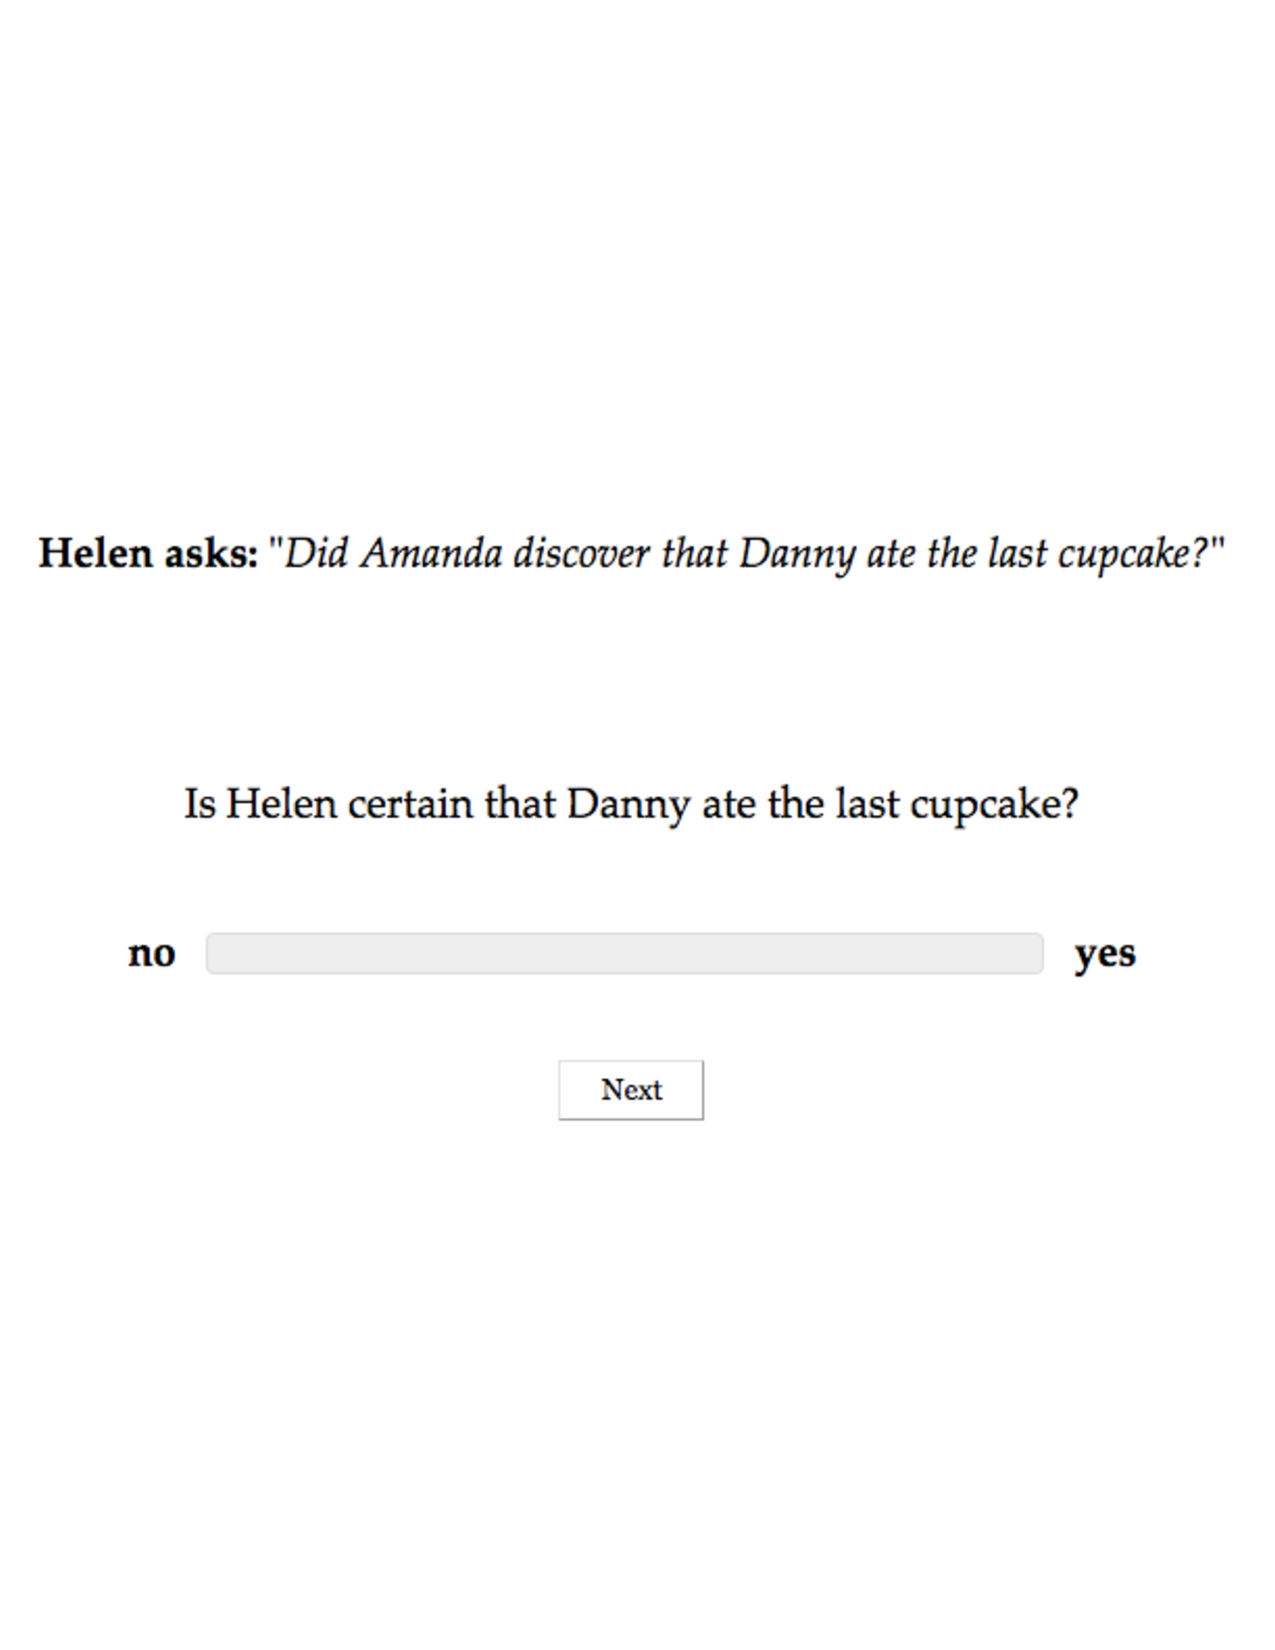
\includegraphics[width=10cm]{figures/trial-exp1}}
\end{center}
\caption{A sample trial in Experiment 1}\label{fig-trial-exp1}
\end{figure}

After completing the experiment, participants filled out a short, optional survey about their age, their gender, their native language(s) and, if English is their native language, whether they are a speaker of American English (as opposed to, e.g., Australian or Indian English). To encourage them to respond truthfully, participants were told that they would be paid no matter what answers they gave in the survey.

\paragraph{Data exclusion}
Prior to analysis, the data from 13 participants who did not self-identify as native speakers of American English were excluded. To assess whether the remaining 287 participants attended to the task, we inspected their responses to the 6 control stimuli, for which we expected low responses. We excluded the data from 16 participants whose response means on the controls were more than 2 standard deviations above the group mean. We furthermore identified 5 participants whose variance in overall response distribution was more than 2 standard deviations below the mean by-participant variance: these participants always selected roughly the same point on the response scale. We excluded the data from these 5 participants, too, leaving data from 266 participants (ages 20-71; median: 36; 118 female, 143 male, 2 other, 3 undeclared).

\subsubsection{Results and discussion}\label{s22}

Figure \ref{f-projectivity} shows the mean certainty ratings for the target stimuli by predicate as well as for the main clause stimuli (abbreviated `MC'), in increasing order from left to right. The mean certainty ratings are largely consistent with impressionistic judgments reported in the literature: First, the ratings for main clause content are lowest overall, as expected for non-projective content. Second, the ratings for factive predicates are among the highest overall, suggesting comparatively high projectivity of the CC. Third, the mean certainty ratings of many optionally factive predicates are lower than those of many factive predicates and higher than those of main clauses as well as of non-veridical non-factives. However, Figure \ref{f-projectivity} also shows that the CCs of the 5 predicates assumed to be factive are not categorically more projective than the CCs of the optionally factive predicates, contrary to what is expected under the first definition of factive predicates. Specifically, the CCs of the optionally factive predicates {\em acknowledge, hear} and {\em inform} are at least as projective as the CCs of {\em reveal} or {\em discover}. This finding suggests that projectivity alone does not categorically distinguish factive predicates from optionally factive and non-factive ones.

\begin{figure}[H]
\centering

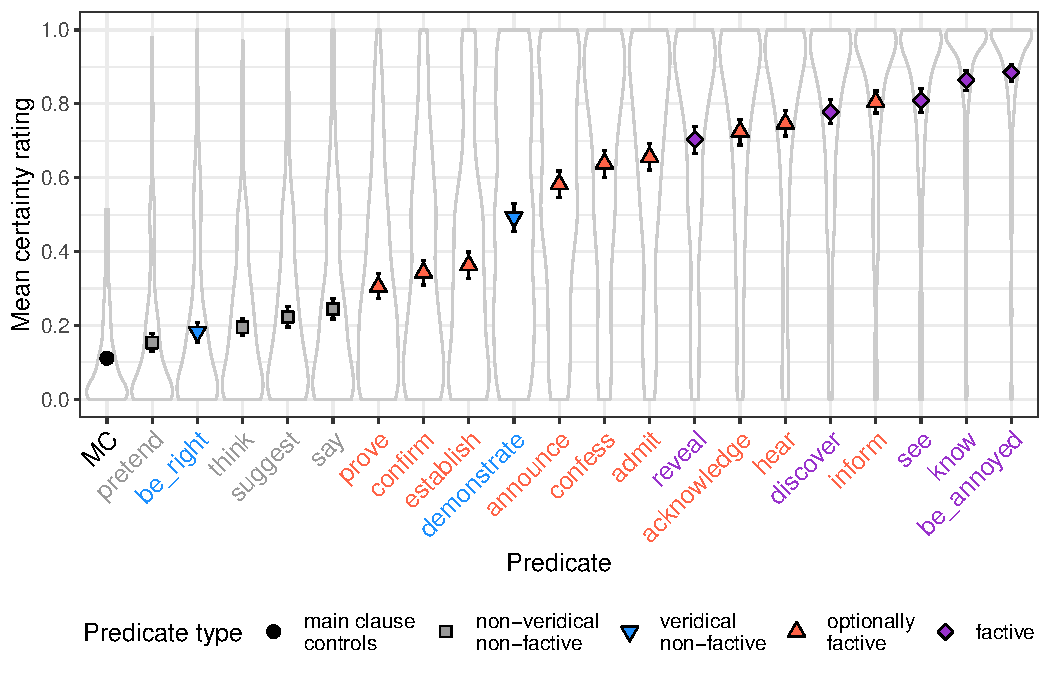
\includegraphics[width=.7\paperwidth]{../../results/5-projectivity-no-fact/graphs/means-projectivity-by-predicate-variability}

\caption{Mean certainty ratings by predicate. Error bars indicate 95\% bootstrapped confidence intervals. Light gray dots indicate individual participants' responses.} %Factive predicates are given in purple, veridical non-factive ones in blue, non-veridical non-factive ones in gray and optionally factive ones in orange.  `MC' abbreviates main clause stimuli.}
\label{f-projectivity}
\end{figure}




%1 acknowledge 0.725 0.0330  0.0339  0.692 0.758
% 2 admit       0.656 0.0390  0.0352  0.617 0.691
% 3 announce    0.582 0.0375  0.0370  0.545 0.619
% 4 be_annoyed  0.885 0.0220  0.0226  0.863 0.907
% 5 be_right    0.183 0.0271  0.0251  0.155 0.208
% 6 confess     0.639 0.0399  0.0376  0.599 0.676
% 7 confirm     0.343 0.0350  0.0358  0.308 0.379
% 8 MC          0.111 0.00895 0.00860 0.102 0.120
% 9 demonstrate 0.493 0.0403  0.0382  0.452 0.531
%10 discover    0.779 0.0303  0.0308  0.748 0.809
%11 establish   0.363 0.0340  0.0404  0.329 0.403
%12 hear        0.747 0.0371  0.0360  0.710 0.783
%13 inform      0.805 0.0287  0.0305  0.776 0.836
%14 know        0.864 0.0269  0.0241  0.837 0.888
%15 pretend     0.153 0.0232  0.0276  0.130 0.181
%16 prove       0.305 0.0314  0.0289  0.273 0.334
%17 reveal      0.704 0.0377  0.0349  0.666 0.739
%18 say         0.245 0.0283  0.0287  0.216 0.273
%19 see         0.809 0.0330  0.0303  0.776 0.840
%20 suggest     0.223 0.0256  0.0253  0.197 0.248
%21 think       0.195 0.0236  0.0243  0.172 0.220


One might ask whether the categorization of clause-embedding predicates assumed in (\ref{pred}) is correct and whether there is a different place in which a line can be drawn between factive and optionally factive predicates based on the projectivity of the CCs. The mean certainty ratings plotted in Figure \ref{f-projectivity} suggest that this cannot be done in a non-arbitrary way. For instance, one might consider all predicates factive whose CC is at least as projective as that of {\em reveal}: this would mean that the predicates typically taken to be factive are factive, as well as {\em acknowledge, hear} and {\em inform}. There is, however, no principled reason why the projectivity of the CC of {\em reveal} should be the cut-off for factivity. A different approach would be to pick an arbitrary mean certainty rating, say .8, and to categorize predicates whose CC has a mean certainty rating of at least .8 as factive and predicates whose CC has a mean certainty rating below .8 as optionally factive. However, this is as unprincipled an approach as the previous one -- one could just as well pick a threshold of .85 or .75, with the result that different predicates would be considered factive: for instance, {\em discover} (mean: .78) would not count as factive with a threshold of .8, but would with a threshold of .75, and {\em see} (mean: .81) would count as factive with a threshold of .8, but not with a threshold of .85.\footnote{Choosing an arbitrary numeric threshold for factivity is also complicated by the fact that there is by-experiment variation in mean certainty ratings. For instance, the mean certainty ratings in Exp.~1a were lower, overall, than the mean certainty ratings in \citetpos{tbd-variability} Exps.~1. For example, the CC of {\em be annoyed}, which was the most projective in both sets of experiments, received mean certainty ratings of .96  and .92 in \citetpos{tbd-variability} Exps.~1a and 1b, respectively, but only a .86 in our Exp.~1a. This difference may be due to the fact that \citet{tbd-variability} primarily investigated highly projective content whereas our Exp.~1a included a wide range of less projective content: it is possible that participants' certainty ratings were influenced by the overall projectivity of the contents investigated. We leave this matter to future research.}

The possibility of categorizing clause-embedding predicates by the projectivity of the CC is further called into question by the fact that the CC of all of the 20 predicates investigated is projective, albeit to varying degrees, compared to the non-projective main clause controls. This was established by fitting a zero-one-inflated Beta (ZOIB) regression model \citep{liu2015} with weakly informative priors using the \verb|brms| \citep{buerkner2017}  package in R \citep{R}. The model predicted the certainty ratings from a fixed effect of predicate (with treatment coding and `main clause' as  reference level) and included the maximal random effects structure justified by the design: random by-participant and by-content intercepts and random by-participant and by-content slopes for the fixed effect of predicate (capturing random variability in overall projectivity by content and participant as well as random variability in the effect of predicate, which may vary by participant and content).\footnote{For details on the ZOIB model see Appendix \ref{a-zoib}\jd{create}} 

Mean certainty ratings for all predicates were higher than for the main clause controls \jd{use hypothesis() to establiish? also: need to adjust if, eg, say doesn't come out as different. one way of doing this: table of posterior p(predicate $>$ MC), maybe show plots in appendix?}, suggesting that the CC of \jd{all?} predicates is at least weakly projective.  {\bf DESCRIBE FINDINGS FOR LEAST PROJECTIVE PREDICATES?} 

In sum, speakers who utter an interrogative with one of the 20 clause-embedding predicates are taken to be more committed to the CC than to the main clause control content.\footnote{According to \citet[1739]{spector-egre2015}, it is not clear whether the CC of {\em say} is projective. Our Exp.~1a findings suggest that it is weakly projective.}    Thus, to distinguish factive predicates from optionally factive and non-factive ones in this set of 20 predicates, one would need to distinguish one group of projective CCs from another group of projective CCs. The results suggest that there is no principled way of doing so.


{\bf APPENDIX:} 

\begin{itemize}

\item give more general explanation of why a ZOIB model is appropriate for these data, 

\item Four chains converged after 2000 iterations each (warmup = 1000, \(\hat{R}=1\) for all estimated parameters).

\item In order to evaluate the evidence for an effect of the at-issueness of the generalization, we report 95\% credible intervals and the posterior probability $P(\beta > 0)$ that the at-issueness coefficient $\beta$ is greater than zero. A 95\% credible interval (CI) demarcates the range of values that comprise 95\% of probability mass of our posterior beliefs such that no value inside the CI has a lower probability than any point outside it \citep{Jaynes1976, Morey2016}. There is substantial evidence for an effect if zero is (by a reasonably clear margin) not included in the 95\% CI and $P(\beta > 0)$ is close to zero or one. Posterior probabilities tell us the probability that the parameter has a certain value, given the data and model (these probabilities are not frequentist $p$-values). In order to present statistics as close to widely used frequentist practices, and following \citealt{Nicenboim2016}, we defined an inferential criterion that seems familiar (95\%), but the strength of evidence should not be taken as having clear cut-off points (such as in a null-hypothesis significance testing framework).

\item The model provided evidence for the predicted effect of the at-issueness of the generalization on the at-issueness of the prejacent: the prejacent of EASs for which the truth of the generalizations was more likely to follow from the common ground were more likely to receive a `yes' (at-issue) rating than the prejacent of EAS for which the truth of the generalization was less likely to follow from the common ground  (posterior mean $\beta$ = 1.29, 95\% CI={[}0.69,1.87{]}, $P(\beta > 0)$ = 1). This finding suggests that the prejacent of EASs is more at-issue when the generalization is less at-issue than when the generalization is more at-issue, as predicted by the analysis in section \ref{s2}.

\end{itemize}

\jd{add additional discussion from general discussion?}

\subsubsection{Limitations of Exp.~1a}

It is possible that providing participants with a gradient scale encouraged them to provide non-categorical answers, and that the observed projection variability and associated difficulty of drawing a clear line between factive and other predicates is thus an artifact of the task. A categorical distinction might more clearly emerge if participants indicated the speaker's certainty via a categorical rather than a continuous task. To assess this possibility, we conducted Exp.~1b, which was identical to Exp.~1a but employed a two-alternative forced choice task.

\subsection{Experiment 1b: Categorical projection ratings}

\subsubsection{Methods}

\paragraph{Participants} 600 participants with U.S.\ IP addresses and at least 99\% of previous HITs approved were recruited on Amazon's Mechanical Turk platform. They were paid \$1.00 for participating in the experiment.\jd{why were they paid more for this experiment than the slider experiment?}


\paragraph{Materials and procedure} The materials and procedure were identical to those of Exp.~1a, with the exception of the task: participants responded `yes' or `no' to the question of whether the speaker is certain of the relevant content. \jd{can we include screenshot?}

\paragraph{Data exclusion} Prior to analysis, we excluded the data from participants who did not self-identify as native speakers of American English. If a participant took an experiment more than once, we only analyzed the data from the first time they took the experiment \jd{how many?}. We also excluded the data from participants who gave a wrong rating to at least one control\jd{oh, i see, the impossibility of using mc as reference level was built-in! can't we just instead exclude anyone who gave a wrong response on at least 2 controls, that way we can at least get a reasonable estimate of the mc error rate which will generally inform the random effects estimates?}: a rating was considered wrong if it was a `yes' rating on a projectivity control. The data from 426 participants (ages 18-81; median: 37; 200 female, 220 male, 2 other) entered the analysis below. 

\subsubsection{Results and discussion}

Figure \ref{f-projectivity2} shows the proportion of `yes' ratings (indicating projection) for the predicates and the main clause stimuli, in increasing order from left to right. Jittered gray dots indicate the 426 individual participants' ratings. The order of predicates according to the projectivity of their CC in Exp.~1b is strikingly similar to that of Exp.~1a, as evidenced by the very high Spearman rank correlation of .983 (see Appendix \ref{a-binary} for a visualization).\footnote{The Spearman rank correlation coefficient, a value between -1 and 1, is a nonparametric measure of rank correlation: the higher the coefficient, the more the relation between the the two variables can be described using a monotonic function; if the coefficient is positive, the value of one variable tends to increase with an increase in the other. In the case of our experiments, a coefficient of 1 would mean that there is a perfectly monotone increasing relation between the ranking of the predicates in Exp.~1a and Exp.~1b: for any two predicates $p_1$ and $p_2$, if $p_1$ ranks below $p_2$ in Exp.~1a (that is, the mean certainty rating of $p_1$ is lower than that of $p_2$), then that ranking is preserved in Exp.~1b.} 

The critical findings of Exp.~1a were replicated. First, the CCs of the factive predicates were not categorically more projective than the CCs of the optionally factive predicates:  the CCs of {\em acknowledge, hear} and {\em inform} were at least as projective as the CCs of {\em reveal} or {\em discover}. Second, a non-arbitrary line between factive and optionally factive predicates cannot be drawn, as the CC of all factive and optionally factive predicates were projective compared to the non-projective main clause controls \jd{insert model info here once issue of exclusions settled} (for details on the model that was fitted, see Appendix \ref{a-binary}). Thus, like Exp.~1a, the results of Exp.~1b do not support the assumption that factive predicates are categorically distinguished from optionally factive and non-factive ones by the projectivity of the CC alone. 

\begin{figure}[H]

\centering
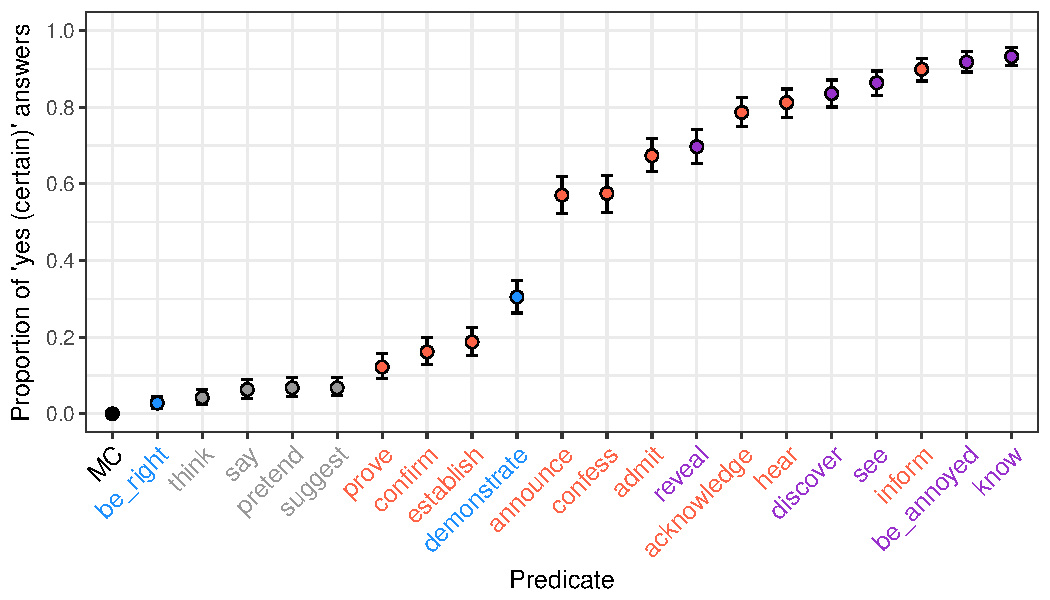
\includegraphics[width=.7\paperwidth]{../../results/8-projectivity-no-fact-binary/graphs/proportion-by-predicate-variability}
\caption{Proportion of `yes' ratings by predicate, collapsing over complement clauses, with 95\% bootstrapped confidence intervals. Factive predicates are given in purple, veridical non-factive ones in blue, non-veridical non-factive ones in gray and optionally factive ones in orange. `MC' abbreviates main clause.}\label{f-projectivity2}

\end{figure}


\subsection{Converging evidence for failure of projection-based definition of factivity}

Converging evidence for the impossibility of establishing a purely projection-based definition of factivity comes from two additional datasets. First, as shown in Figure \ref{f-commitmentbank}, \citet*{demarneffe-etal-sub23} found that factive predicates did not receive categorically higher mean certainty ratings than optionally factive predicates in the CommitmentBank, a collection of naturally occurring discourses with clause-embedding predicates embedded under a variety of entailment-canceling operators.\footnote{We re-plotted their data, obtained at \jd{xxx insert link}} {\bf I THINK ITS GOOD TO INCLUDE A VERSION OF THIS FIGURE.  Of our 20 predicates, only 9 (announce, know, admit, hear, prove, say, see, think, pretend) are included, so I would like to suggest color coding all of the predicates, unlike what we do for MegaVeridicality.} \jd{is there a reason the marneffe et al dataset is described in much less detail than the white and rawlins dataset? either equally little detail on both, or equally much detail on both would be better}

\begin{figure}[H]
\centering
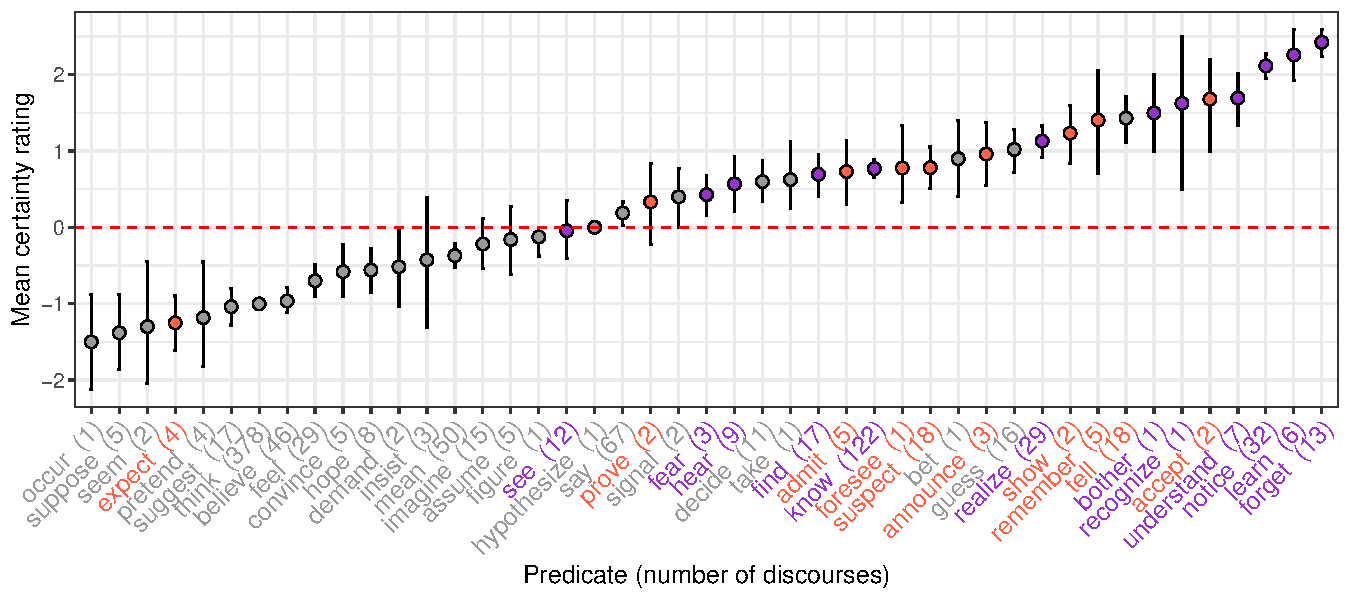
\includegraphics[width=.75\paperwidth]{figures/3-way-means-projectivity-by-predicate-variability}

\caption{Mean certainty ratings by predicate for the predicates in \citet*{demarneffe-etal-sub23} dataset, which includes 9 of the 20 predicates we tested in Exps.1a and 1b \jd{can you make axis labels for the ones we have bold?}. Error bars indicate 95\% bootstrapped confidence intervals. \jd{need to say sth about the scale and the red line -- why does it go from -2 to +2?} \jd{better to include legend like the one i made for figs 2 and 3 instead of writing it in caption -- i can do it if you point me to the code }}%Factive predicates are given in purple, veridical non-factive ones in blue, non-veridical non-factive ones in gray and optionally factive ones in orange. `MC' abbreviates main clause stimuli. X-axis labels for 19 of the 20 predicates featured in our Exps.~1 and 2: factive predicates in purple, the veridical non-factive one in blue, non-veridical non-factive ones in gray and optionally factive ones in orange.}
\label{f-commitmentbank}
\end{figure}

A second piece of converging evidence comes from the MegaVeridicality dataset (\citealt{white-rawlins-nels2018,white-etal2018b}),\footnote{This dataset is  available at \url{http://megaattitude.io.}. The R code of our analysis of the data can be found at  [redacted for review].}
%\url{https://github.com/judith-tonhauser/factivity}.}   
which contains projection ratings for the CCs of 517 English clause-embedding predicates. The stimuli that participants rated consisted of combinations of the 517 predicates with arguments with low lexical content, as shown in (\ref{wr-stim-proj}) for the predicate {\em know}: the predicates and their clausal complements were embedded under negation in stimuli like (\ref{wr-stim-proj}a) and under negation and the question operator in stimuli like (\ref{wr-stim-proj}b). To assess projection, participants were asked to respond to the question {\em Did that thing happen?} for stimuli like (\ref{wr-stim-proj}a) and to respond to the question posed by stimuli like (\ref{wr-stim-proj}b). The response options were `yes', `maybe or maybe not' and `no'. 

\begin{exe}
\ex\label{wr-stim-proj}
\begin{xlist}
\ex Somebody didn't know that a particular thing happened.
\ex If somebody didn't know that a particular thing happened, did that thing happen?
\end{xlist}
\end{exe}

Each of the 517 predicates in the MegaVeridicality dataset received between 29 and 60 projectivity ratings (mean: 32) from a total of 290 participants. To plot the ratings and to compare them to the findings of our experiments, we coded a `yes' response as 1,  a `maybe or maybe not' response as 0 and a `no' response as -1.\footnote{We assume that a `maybe or maybe not' response means that the participant is not certain whether the CC is true (i.e., whether that thing happened) and that a `no' response means that the CC is false (i.e., that thing did not happen). Thus, for ease of comparison with our data, a `maybe or maybe not' response was coded as 0.} Figure \ref{f-white-rawlins-projectivity} plots the mean projectivity ratings for the 517 predicates in the MegaVeridicality dataset, with x-axis labels for 19 of the 20 predicates that we investigated (the predicate {\em be right} is not included in the MegaVeridicality dataset). As shown,\footnote{The x-axis labels for the following predicates overlap: {\em discover/confirm} and {\em acknowledge/say/admit}.\jd{better to handle this in a more elegant way in the plot directly}} projectivity does not categorically distinguish factive predicates from optionally factive and non-factive ones: the CCs of the optionally factive predicates {\em confess, acknowledge, announce, hear} and {\em inform} are at least as projective as those of some factive predicates. 

\begin{figure}[H]
\centering
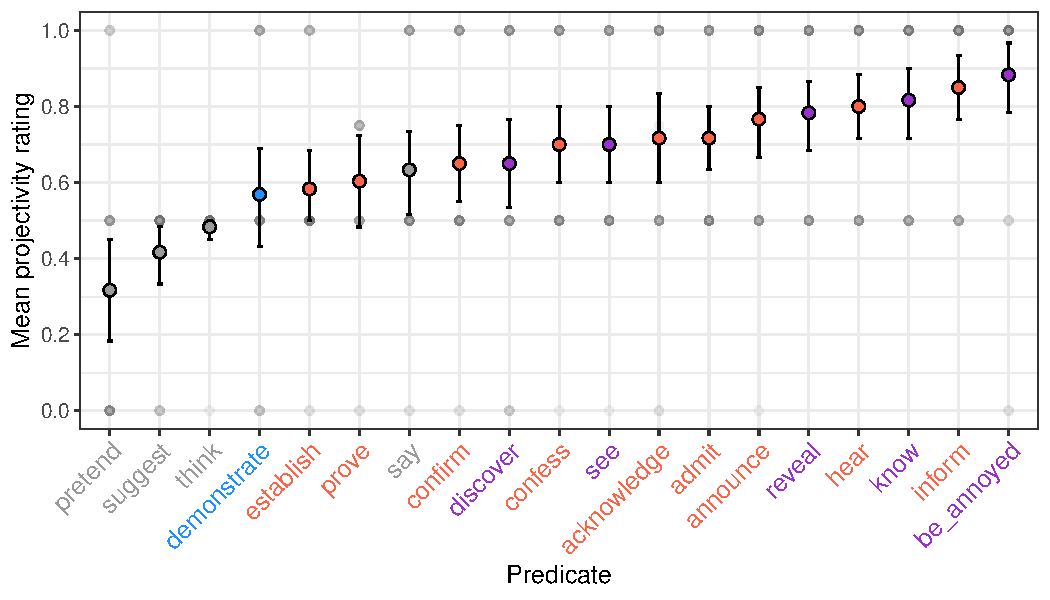
\includegraphics[width=.75\paperwidth]{../../white-rawlins-data/graphs/means-projection-by-predicate}

\caption{Mean projectivity rating in blue, by predicate, with 95\% bootstrapped confidence intervals, for the 517 predicates in MegaVeridicality dataset. X-axis labels for 19 of the 20 predicates featured in our Exps.~1 and 2: factive predicates in purple, the veridical non-factive one in blue, non-veridical non-factive ones in gray and optionally factive ones in orange.\jd{again, better to include color legend rather than provide color mapping in words}}
\label{f-white-rawlins-projectivity}
\end{figure}

Thus, the MegaVeridicality dataset further confirms the result that projectivity alone does not categorically distinguish factive predicates from optionally factive and non-factive ones, contrary to what is expected under the first definition of factive predicates. \jd{"the first def of factive predicates" sounds weird -- can we just refer back to the two defs in the intro, ie have a numbered list of definitions in the intro?} The experiments described in the next section were designed to explore whether the more complex definition of factive predicates (\jd{refer back to the second item in list introduced in intro, see comment above}) according to which entailment and projectivity jointly categorize clause-embedding predicates,  is empirically supported. To this end, we collected entailment judgments for CCs of the same 20 predicates studied in Exps.~1.

%\begin{table}[h!]
%\setlength\tabcolsep{3pt}
%
%\centering
%\small
%
%\begin{tabular}{l l l l l l l l l l l l l l l l l l l l l }
%\toprule
%
%& \rot{{MC}} &   \rot{\color{gray}{\em pretend}\color{black}} & \rot{\color{blue}{\em be right}\color{black}} & \rot{\color{gray}{\em think}\color{black}} &  \rot{\color{gray}{\em suggest}\color{black}} &  \rot{\color{gray}{\em say}\color{black}} & \rot{\color{orange}{\em prove}\color{black}} & \rot{\color{orange}{\em confirm}\color{black}} & \rot{\color{orange}{\em establish}\color{black}} & \rot{\color{blue}{\em demonstrate}\color{black}} & \rot{\color{orange}{\em announce}\color{black}} &\rot{\color{orange}{\em confess}\color{black}}& \rot{\color{orange}{\em admit}\color{black}} & \rot{\color{violet}{\em reveal}\color{black}}  &\rot{\color{orange}{\em acknowledge}\color{black}}  & \rot{\color{orange}{\em hear}\color{black}}  & \rot{\color{violet}{\em discover}\color{black}} & \rot{\color{orange}{\em inform}\color{black}}  & \rot{\color{violet}{\em see}\color{black}}  & \rot{\color{violet}{\em know}\color{black}}  \\
%
%\midrule
%
%\color{gray}{\em pretend}\color{black}	&  n.s. & - & - & - & - & - & - & - & - & - & - & - & - & - & - & - & - & - & - \\
%\color{blue}{\em be right}\color{black}	& . & n.s. & - & - & - & - & - & - & - & - & - & - & - & - & - & - & - & - & - & - \\
%\color{gray}{\em think}\color{black}		& ** & n.s. & n.s. & - & - & - & - & - & - & - & - & - & - & - & - & - & - & - & - & - \\
%\color{gray}{\em suggest}\color{black}	& ***	& n.s. & n.s. & n.s. & - & - & - & - & - & - & - & - & - & - & - & - & - & - & - & - \\
%\color{gray}{\em say}	\color{black}	& ***	& ** & n.s. & n.s. & n.s. & - & - & - & - & - & - & - & - & - & - & - & - & - & - & - \\
%\color{orange}{\em prove}\color{black}		& ***	& *** &  ***  & ** & * & n.s. & - & - & - & - & - & - & - & - & - & - & - & - & - & - \\
%\color{orange}{\em confirm}\color{black}	&***	& ***  &  ***  &  ***  &  ***  & ** & n.s. & - & - & - & - & - & - & - & - & - & - & - & - & - \\
%\color{orange}{\em establish}\color{black}	&***	&  ***  &  ***  &  ***  &  ***  &  ***  & n.s & n.s. & - & - & - & - & - & - & - & - & - & - & - & - \\
%\color{blue}{\em demonstrate}\color{black} &*** & *** & *** & *** &  *** &  *** &  ***  &  ***  &  ***  & - & - & - & - & - & - & - & - & - & - & - \\
%\color{orange}{\em announce}\color{black}		& ***	& *** & *** & *** & *** & *** & *** &  ***  &  ***  & ** & - & - & - & - & - & - & - & - & - & - \\
%\color{orange}{\em confess}\color{black}	& ***	& *** & *** & *** & *** & *** & *** & *** & *** &  ***  & n.s. & - & - & - & - & - & - & - & - & - \\
%\color{orange}{\em admit}\color{black}		& ***	& *** & *** & *** & *** & *** & *** & *** & *** &  ***  & . & n.s. &  - & - & - & - & - & - & - & - \\
%\color{violet}{\em reveal}\color{black}			& ***	& *** & *** & *** & *** & *** & *** & *** & *** &  ***  &  ***  & n.s. & n.s. & - & - & - & - & - & - & - \\
%\color{orange}{\em acknowledge}\color{black}	& ***	& *** & *** & *** & *** & *** & *** & *** & *** &  ***  &  ***  & * & n.s. & n.s. & - & - & - & - & - & - \\
%\color{orange}{\em hear}\color{black}		& ***	& *** & *** & *** & *** & *** & *** & *** & *** & *** &  ***  &  **  & ** & n.s. & n.s. & - & - & - & - & - \\
%\color{violet}{\em discover}\color{black}	& ***		& *** & *** & *** & *** & *** & *** & *** & *** & *** &  ***  &  ***  &  ***  & . & n.s. & n.s. & - & - & - & - \\
%\color{orange}{\em inform}\color{black}		&***		& *** & *** & *** & *** & *** & *** & *** & *** & *** & *** & *** &  ***  & ** & * & n.s. & n.s. & - & - & - \\
%\color{violet}{\em see}\color{black}		&***		& *** & *** & *** & *** & *** & *** & *** & *** & *** & *** &  ***  &  ***  &  ***  & * & n.s. & n.s. & n.s. & - & - \\
%\color{violet}{\em know}\color{black}		&***		& *** & *** & *** & *** & *** & *** & *** & *** & *** & *** & *** & *** & *** & *** & *** & * & n.s. & n.s. & -  \\
%\color{violet}{\em be annoyed}\color{black}	&***		& *** & *** & *** & *** & *** & *** & *** & *** & ***  & ***  & *** & *** & *** & *** & *** & ** & * & . & ns  \\
%
%\bottomrule
%\end{tabular}
%\caption{P-values associated with pairwise comparisons of certainty ratings of the 20 clause-embedding predicates and the main clause controls using Tukey's method. `***' indicates significance at .0001, `**' at .01, `*' at .05, `.' marginal significance at .1, and `n.s' indicates no significant difference in means. `MC' abbreviates main clause controls. Factive predicates are given in purple, optionally factive ones in orange, veridical non-factive ones in lighter blue and non-veridical non-factive ones in grey.}\label{t-pairwise-proj}
%\end{table} 
%

%# contrast                      estimate         SE     df t.ratio p.value
%# MC - pretend              -0.042020639 0.01916977  49.97  -2.192  0.8098
%# MC - be_right             -0.071607572 0.01916501  50.13  -3.736  0.0542
%# MC - think                -0.083783582 0.01916492  50.07  -4.372  0.0089
%# MC - suggest              -0.111608001 0.01912903  50.69  -5.834  0.0001
%# MC - say                  -0.133890950 0.01912899  50.72  -6.999  <.0001
%# MC - prove                -0.193307193 0.01914129  50.50 -10.099  <.0001
%# MC - confirm              -0.231812154 0.01917434  50.04 -12.090  <.0001
%# MC - establish            -0.251595754 0.01913785  50.56 -13.146  <.0001
%# MC - demonstrate          -0.381538510 0.01913109  50.66 -19.943  <.0001
%# MC - announce             -0.471695123 0.01912825  50.73 -24.660  <.0001
%# MC - confess              -0.527021744 0.01916157  50.13 -27.504  <.0001
%# MC - admit                -0.544807503 0.01912812  50.71 -28.482  <.0001
%# MC - reveal               -0.592362151 0.01912462  50.78 -30.974  <.0001
%# MC - acknowledge          -0.613560616 0.01916529  50.13 -32.014  <.0001
%# MC - hear                 -0.634910506 0.01912981  50.72 -33.190  <.0001
%# MC - discover             -0.667312302 0.01913513  50.63 -34.874  <.0001
%# MC - inform               -0.693266524 0.01915643  50.26 -36.190  <.0001
%# MC - see                  -0.697664502 0.01914503  50.43 -36.441  <.0001
%# MC - know                 -0.752791183 0.01913805  50.55 -39.335  <.0001
%# MC - be_annoyed           -0.773522289 0.01915574  50.30 -40.381  <.0001

%# pretend - be_right        -0.029586933 0.02175318 352.08  -1.360  0.9989
%# pretend - think           -0.041762942 0.02175315 351.11  -1.920  0.9404
%# pretend - suggest         -0.069587361 0.02172153 363.43  -3.204  0.1553
%# pretend - say             -0.091870311 0.02172148 363.91  -4.229  0.0051
%# pretend - prove           -0.151286554 0.02173230 359.55  -6.961  <.0001
%# pretend - confirm         -0.189791515 0.02176139 349.96  -8.721  <.0001
%# pretend - establish       -0.209575115 0.02172928 360.73  -9.645  <.0001
%# pretend - demonstrate     -0.339517871 0.02172331 362.84 -15.629  <.0001
%# pretend - announce        -0.429674484 0.02172086 363.99 -19.782  <.0001
%# pretend - confess         -0.485001104 0.02175018 352.32 -22.299  <.0001
%# pretend - admit           -0.502786864 0.02172074 363.80 -23.148  <.0001
%# pretend - reveal          -0.550341512 0.02171763 365.20 -25.341  <.0001
%# pretend - acknowledge     -0.571539977 0.02175347 351.98 -26.274  <.0001
%# pretend - hear            -0.592889867 0.02172222 363.73 -27.294  <.0001
%# pretend - discover        -0.625291662 0.02172689 361.93 -28.780  <.0001
%# pretend - inform          -0.651245884 0.02174563 354.69 -29.948  <.0001
%# pretend - see             -0.655643862 0.02173562 358.16 -30.164  <.0001
%# pretend - know            -0.710770543 0.02172942 360.62 -32.710  <.0001
%# pretend - be_annoyed      -0.731501649 0.02174507 355.26 -33.640  <.0001

%# be_right - think          -0.012176009 0.02174894 353.91  -0.560  1.0000
%# be_right - suggest        -0.040000428 0.02171732 366.37  -1.842  0.9600
%# be_right - say            -0.062283378 0.02171730 366.84  -2.868  0.3344
%# be_right - prove          -0.121699621 0.02172813 362.42  -5.601  <.0001
%# be_right - confirm        -0.160204582 0.02175720 352.72  -7.363  <.0001
%# be_right - establish      -0.179988182 0.02172509 363.62  -8.285  <.0001
%# be_right - demonstrate    -0.309930938 0.02171914 365.74 -14.270  <.0001
%# be_right - announce       -0.400087551 0.02171664 366.95 -18.423  <.0001
%# be_right - confess        -0.455414171 0.02174594 355.15 -20.942  <.0001
%# be_right - admit          -0.473199931 0.02171652 366.75 -21.790  <.0001
%# be_right - reveal         -0.520754579 0.02171338 368.20 -23.983  <.0001
%# be_right - acknowledge    -0.541953044 0.02174927 354.77 -24.918  <.0001
%# be_right - hear           -0.563302934 0.02171802 366.67 -25.937  <.0001
%# be_right - discover       -0.595704730 0.02172270 364.85 -27.423  <.0001
%# be_right - inform         -0.621658951 0.02174146 357.50 -28.593  <.0001
%# be_right - see            -0.626056929 0.02173140 361.04 -28.809  <.0001
%# be_right - know           -0.681183610 0.02172529 363.46 -31.354  <.0001
%# be_right - be_annoyed     -0.701914716 0.02174087 358.10 -32.285  <.0001

%# think - suggest           -0.027824419 0.02171720 365.42  -1.281  0.9995
%# think - say               -0.050107369 0.02171718 365.89  -2.307  0.7508
%# think - prove             -0.109523612 0.02172804 361.46  -5.041  0.0001
%# think - confirm           -0.148028572 0.02175712 351.80  -6.804  <.0001
%# think - establish         -0.167812173 0.02172500 362.66  -7.724  <.0001
%# think - demonstrate       -0.297754928 0.02171905 364.77 -13.709  <.0001
%# think - announce          -0.387911542 0.02171658 365.95 -17.862  <.0001
%# think - confess           -0.443238162 0.02174589 354.19 -20.383  <.0001
%# think - admit             -0.461023921 0.02171643 365.78 -21.229  <.0001
%# think - reveal            -0.508578569 0.02171334 367.18 -23.422  <.0001
%# think - acknowledge       -0.529777035 0.02174921 353.82 -24.358  <.0001
%# think - hear              -0.551126924 0.02171787 365.74 -25.377  <.0001
%# think - discover          -0.583528720 0.02172260 363.89 -26.863  <.0001
%# think - inform            -0.609482942 0.02174134 356.58 -28.033  <.0001
%# think - see               -0.613880920 0.02173129 360.11 -28.249  <.0001
%# think - know              -0.669007601 0.02172518 362.52 -30.794  <.0001
%# think - be_annoyed        -0.689738707 0.02174078 357.16 -31.726  <.0001

%# suggest - say             -0.022282950 0.02168553 379.04  -1.028  1.0000
%# suggest - prove           -0.081699192 0.02169639 374.37  -3.766  0.0285
%# suggest - confirm         -0.120204153 0.02172556 364.09  -5.533  <.0001
%# suggest - establish       -0.139987753 0.02169334 375.64  -6.453  <.0001
%# suggest - demonstrate     -0.269930509 0.02168737 377.89 -12.446  <.0001
%# suggest - announce        -0.360087123 0.02168490 379.13 -16.605  <.0001
%# suggest - confess         -0.415413743 0.02171425 366.68 -19.131  <.0001
%# suggest - admit           -0.433199502 0.02168475 378.95 -19.977  <.0001
%# suggest - reveal          -0.480754150 0.02168168 380.41 -22.173  <.0001
%# suggest - acknowledge     -0.501952616 0.02171755 366.31 -23.113  <.0001
%# suggest - hear            -0.523302505 0.02168625 378.86 -24.131  <.0001
%# suggest - discover        -0.555704301 0.02169097 376.91 -25.619  <.0001
%# suggest - inform          -0.581658523 0.02170974 369.17 -26.793  <.0001
%# suggest - see             -0.586056501 0.02169969 372.89 -27.008  <.0001
%# suggest - know            -0.641183182 0.02169352 375.49 -29.556  <.0001
%# suggest - be_annoyed      -0.661914288 0.02170912 369.83 -30.490  <.0001

%# say - prove               -0.059416243 0.02169635 374.86  -2.739  0.4254
%# say - confirm             -0.097921204 0.02172555 364.55  -4.507  0.0016
%# say - establish           -0.117704804 0.02169334 376.11  -5.426  <.0001
%# say - demonstrate         -0.247647560 0.02168737 378.36 -11.419  <.0001
%# say - announce            -0.337804173 0.02168484 379.66 -15.578  <.0001
%# say - confess             -0.393130793 0.02171422 367.16 -18.105  <.0001
%# say - admit               -0.410916553 0.02168471 379.46 -18.950  <.0001
%# say - reveal              -0.458471201 0.02168165 380.91 -21.146  <.0001
%# say - acknowledge         -0.479669666 0.02171752 366.79 -22.087  <.0001
%# say - hear                -0.501019556 0.02168617 379.41 -23.103  <.0001
%# say - discover            -0.533421352 0.02169092 377.43 -24.592  <.0001
%# say - inform              -0.559375573 0.02170970 369.66 -25.766  <.0001
%# say - see                 -0.563773551 0.02169966 373.39 -25.981  <.0001
%# say - know                -0.618900232 0.02169349 375.98 -28.529  <.0001
%# say - be_annoyed          -0.639631338 0.02170909 370.31 -29.464  <.0001

%# prove - confirm           -0.038504961 0.02173640 360.15  -1.771  0.9731
%# prove - establish         -0.058288561 0.02170419 371.50  -2.686  0.4651
%# prove - demonstrate       -0.188231317 0.02169820 373.73  -8.675  <.0001
%# prove - announce          -0.278387930 0.02169568 374.99 -12.831  <.0001
%# prove - confess           -0.333714550 0.02172508 362.71 -15.361  <.0001
%# prove - admit             -0.351500310 0.02169558 374.77 -16.201  <.0001
%# prove - reveal            -0.399054958 0.02169251 376.20 -18.396  <.0001
%# prove - acknowledge       -0.420253423 0.02172836 362.36 -19.341  <.0001
%# prove - hear              -0.441603313 0.02169707 374.69 -20.353  <.0001
%# prove - discover          -0.474005109 0.02170182 372.75 -21.842  <.0001
%# prove - inform            -0.499959330 0.02172053 365.19 -23.018  <.0001
%# prove - see               -0.504357308 0.02171049 368.84 -23.231  <.0001
%# prove - know              -0.559483989 0.02170436 371.35 -25.777  <.0001
%# prove - be_annoyed        -0.580215095 0.02171994 365.81 -26.713  <.0001

%# confirm - establish       -0.019783600 0.02173331 361.39  -0.910  1.0000
%# confirm - demonstrate     -0.149726356 0.02172736 363.49  -6.891  <.0001
%# confirm - announce        -0.239882969 0.02172486 364.68 -11.042  <.0001
%# confirm - confess         -0.295209590 0.02175419 352.98 -13.570  <.0001
%# confirm - admit           -0.312995349 0.02172471 364.51 -14.407  <.0001
%# confirm - reveal          -0.360549997 0.02172167 365.86 -16.599  <.0001
%# confirm - acknowledge     -0.381748462 0.02175744 352.66 -17.546  <.0001
%# confirm - hear            -0.403098352 0.02172625 364.40 -18.554  <.0001
%# confirm - discover        -0.435500148 0.02173092 362.60 -20.041  <.0001
%# confirm - inform          -0.461454369 0.02174966 355.33 -21.217  <.0001
%# confirm - see             -0.465852348 0.02173966 358.81 -21.429  <.0001
%# confirm - know            -0.520979028 0.02173343 361.29 -23.971  <.0001
%# confirm - be_annoyed      -0.541710134 0.02174904 355.95 -24.907  <.0001

%# establish - demonstrate   -0.129942756 0.02169515 375.00  -5.989  <.0001
%# establish - announce      -0.220099369 0.02169266 376.24 -10.146  <.0001
%# establish - confess       -0.275425990 0.02172202 363.93 -12.680  <.0001
%# establish - admit         -0.293211749 0.02169254 376.04 -13.517  <.0001
%# establish - reveal        -0.340766397 0.02168946 377.49 -15.711  <.0001
%# establish - acknowledge   -0.361964862 0.02172535 363.54 -16.661  <.0001
%# establish - hear          -0.383314752 0.02169403 375.97 -17.669  <.0001
%# establish - discover      -0.415716548 0.02169871 374.07 -19.159  <.0001
%# establish - inform        -0.441670769 0.02171751 366.39 -20.337  <.0001
%# establish - see           -0.446068748 0.02170745 370.08 -20.549  <.0001
%# establish - know          -0.501195428 0.02170132 372.61 -23.095  <.0001
%# establish - be_annoyed    -0.521926534 0.02171688 367.05 -24.033  <.0001

%# demonstrate - announce    -0.090156613 0.02168671 378.48  -4.157  0.0068
%# demonstrate - confess     -0.145483234 0.02171609 366.04  -6.699  <.0001
%# demonstrate - admit       -0.163268993 0.02168659 378.27  -7.529  <.0001
%# demonstrate - reveal      -0.210823641 0.02168350 379.75  -9.723  <.0001
%# demonstrate - acknowledge -0.232022106 0.02171937 365.68 -10.683  <.0001
%# demonstrate - hear        -0.253371996 0.02168808 378.19 -11.683  <.0001
%# demonstrate - discover    -0.285773792 0.02169275 376.29 -13.174  <.0001
%# demonstrate - inform      -0.311728014 0.02171154 368.55 -14.358  <.0001
%# demonstrate - see         -0.316125992 0.02170150 372.26 -14.567  <.0001
%# demonstrate - know        -0.371252672 0.02169533 374.84 -17.112  <.0001
%# demonstrate - be_annoyed  -0.391983778 0.02171092 369.20 -18.055  <.0001

%# announce - confess        -0.055326620 0.02171357 367.26  -2.548  0.5718
%# announce - admit          -0.073112380 0.02168406 379.57  -3.372  0.0981
%# announce - reveal         -0.120667028 0.02168102 381.01  -5.566  <.0001
%# announce - acknowledge    -0.141865493 0.02171682 366.93  -6.533  <.0001
%# announce - hear           -0.163215383 0.02168556 379.49  -7.526  <.0001
%# announce - discover       -0.195617179 0.02169026 377.55  -9.019  <.0001
%# announce - inform         -0.221571400 0.02170904 369.77 -10.206  <.0001
%# announce - see            -0.225969378 0.02169903 373.47 -10.414  <.0001
%# announce - know           -0.281096059 0.02169282 376.11 -12.958  <.0001
%# announce - be_annoyed     -0.301827165 0.02170843 370.42 -13.904  <.0001

%# confess - admit           -0.017785759 0.02171345 367.07  -0.819  1.0000
%# confess - reveal          -0.065340407 0.02171039 368.45  -3.010  0.2478
%# confess - acknowledge     -0.086538873 0.02174624 355.04  -3.979  0.0134
%# confess - hear            -0.107888762 0.02171498 366.96  -4.968  0.0002
%# confess - discover        -0.140290558 0.02171962 365.17  -6.459  <.0001
%# confess - inform          -0.166244780 0.02173840 357.79  -7.648  <.0001
%# confess - see             -0.170642758 0.02172837 361.32  -7.853  <.0001
%# confess - know            -0.225769439 0.02172222 363.77 -10.393  <.0001
%# confess - be_annoyed      -0.246500545 0.02173779 358.41 -11.340  <.0001

%# admit - reveal            -0.047554648 0.02168088 380.81  -2.193  0.8226
%# admit - acknowledge       -0.068753113 0.02171675 366.70  -3.166  0.1709
%# admit - hear              -0.090103003 0.02168545 379.27  -4.155  0.0068
%# admit - discover          -0.122504799 0.02169011 377.37  -5.648  <.0001
%# admit - inform            -0.148459021 0.02170898 369.52  -6.839  <.0001
%# admit - see               -0.152856999 0.02169890 373.28  -7.044  <.0001
%# admit - know              -0.207983680 0.02169272 375.88  -9.588  <.0001
%# admit - be_annoyed        -0.228714786 0.02170827 370.26 -10.536  <.0001

%# reveal - acknowledge      -0.021198465 0.02171367 368.09  -0.976  1.0000
%# reveal - hear             -0.042548355 0.02168234 380.77  -1.962  0.9275
%# reveal - discover         -0.074950151 0.02168705 378.81  -3.456  0.0768
%# reveal - inform           -0.100904373 0.02170584 370.99  -4.649  0.0009
%# reveal - see              -0.105302351 0.02169580 374.73  -4.854  0.0003
%# reveal - know             -0.160429031 0.02168964 377.33  -7.397  <.0001
%# reveal - be_annoyed       -0.181160138 0.02170524 371.63  -8.346  <.0001

%# acknowledge - hear        -0.021349890 0.02171823 366.62  -0.983  1.0000
%# acknowledge - discover    -0.053751686 0.02172293 364.79  -2.474  0.6289
%# acknowledge - inform      -0.079705907 0.02174171 357.42  -3.666  0.0400
%# acknowledge - see         -0.084103885 0.02173165 360.97  -3.870  0.0199
%# acknowledge - know        -0.139230566 0.02172545 363.46  -6.409  <.0001
%# acknowledge - be_annoyed  -0.159961672 0.02174108 358.05  -7.358  <.0001

%# hear - discover           -0.032401796 0.02169165 377.25  -1.494  0.9963
%# hear - inform             -0.058356018 0.02171044 369.47  -2.688  0.4634
%# hear - see                -0.062753996 0.02170037 373.22  -2.892  0.3186
%# hear - know               -0.117880676 0.02169422 375.79  -5.434  <.0001
%# hear - be_annoyed         -0.138611782 0.02170981 370.14  -6.385  <.0001

%# discover - inform         -0.025954222 0.02171514 367.61  -1.195  0.9998
%# discover - see            -0.030352200 0.02170507 371.33  -1.398  0.9985
%# discover - know           -0.085478881 0.02169893 373.88  -3.939  0.0154
%# discover - be_annoyed     -0.106209987 0.02171446 368.32  -4.891  0.0003

%# inform - see              -0.004397978 0.02172387 363.74  -0.202  1.0000
%# inform - know             -0.059524659 0.02171765 366.27  -2.741  0.4237
%# inform - be_annoyed       -0.080255765 0.02173323 360.85  -3.693  0.0366

%# see - know                -0.055126681 0.02170760 369.95  -2.540  0.5784
%# see - be_annoyed          -0.075857787 0.02172323 364.40  -3.492  0.0691

%# know - be_annoyed         -0.020731106 0.02171705 366.90  -0.955  1.0000


 
\section{Experiment 2 and 3: Entailment}\label{s3}

Experiments 2 and 3 explored which of the CCs of the 20 clause-embedding predicates are entailed. We assume the standard definition of entailment, according to which entailment is a binary, categorical relation between two contents: given sentences $\phi$ and $\psi$, the content of $\phi$ entails the content of $\psi$ if and only if every world in which the content of $\phi$ is true is also a world in which the content of $\psi$ is true. Thus, if there is even one world in which $\phi$ is true but $\phi$ is false, then the content of $\phi$ does not entail the content of $\psi$. Given this definition, establishing that the contents of two natural language sentences $\phi$ and $\psi$ do not stand in an entailment relation involves identifying a world in which the content of $\phi$ is true and the content of $\psi$ is false. \jd{the following sentence is rhetorically a little weird: aren't we precisely interested in identifying when there \emph{is} an entailment relationship? the way it's framed makes it sound liike we're mostly interested in showing non-entailment. -- more generally, do we need all the detail of this paragraph or can we just move directly to the next paragraph, which introduces the standard diagnostics for entailment?} In this paper, however, we are also interested in establishing that the contents of two sentences $\phi$ and $\psi$  do stand in an entailment relation. Establishing this is straightforward if the content of some expression in $\phi$ denotes a subset of the content of some expression in $\psi$: for instance, in (\ref{ent1}a),  the content of $\phi$ entails the content of $\psi$ because the denotation of {\em black cat} in $\phi$ is a subset of the denotation of {\em cat} in $\psi$. No such structural relation exists, however, between the content of a sentence with a clause-embedding predicate and the CC, as in (\ref{ent1}b). %Furthermore, it is of course impossible to empirically verify that the content of $\phi$ entails the content of $\psi$ in (\ref{ent1}b) because it is impossible to verify that $\psi$ is true in all worlds in which $\phi$ is true. 

\begin{exe}
\ex\label{ent1}
\begin{xlist}
\ex $\phi$: Sam owns a black cat. \hspace*{1.5cm} $\psi$: Sam owns a cat.

\ex $\phi$: Sam knows that it's raining. \hspace*{.6cm} $\psi$: It's raining.

\end{xlist}
\end{exe}

To establish whether the content of an unembedded matrix sentence with a clause-embedding predicate entails the CC, we use standard diagnostics that are taken to provide evidence for an entailment relation. Two standard diagnostics are given in (\ref{diag}). According to the `inference diagnostic' in (\ref{diag}a), the content of an unembedded matrix sentence with a clause-embedding predicate entails the CC if and only if the CC definitely follows from a true statement of the unembedded matrix sentence. According to the `contradictoriness diagnostic' in (\ref{diag}b), an entailment relationship holds if and only an utterance of the unembedded matrix sentence that is followed by a denial of the CC is contradictory. 

\begin{exe}
\ex\label{diag} Two diagnostics for entailment \hfill (see, e.g., \citealt[\S3.1]{ccmg90})
\begin{xlist}
\ex  Inference diagnostic (Exps.~2a and 2b)\\ $\phi$ entails $\psi$ if and only if, if $\phi$ is true, then the truth of $\psi$ definitely follows. 

\ex  Contradictoriness diagnostic  (Exps.~3a and 3b)\\ $\phi$ entails $\psi$ if and only if sentences of the form {\em $\phi$ and not $\psi$} are contradictory. 

\end{xlist}
\end{exe}
These two diagnostics for entailment were applied to the CCs of the 20 clause-embedding predicates in Exps.~2a/2b and Exps.~3a/3b, respectively. The (a) and (b) versions of the experiments differed in whether participants provided a continuous or categorical response.  Both sets of experiments included control stimuli for which the relevant contents stand in an entailment relation, that is, for which the relevant inference definitely follows (Exps.~2) and that are definitely contradictory (Exp.~3). We assume that the CC of a clause-embedding predicate is not entailed if responses to the CC are significantly different from responses to these control stimuli and that the CC of a clause-embedding predicate is entailed if responses to the CC are not significantly different from responses to these control stimuli. Thus, identifying entailed CCs  requires arguing from a null result. 

We present the findings of the two experiments in sections \ref{s31} and \ref{s32}, and then discuss the findings jointly in section \ref{s33} \jd{revise after restructuring}: given the standard classification of the 20 clause-embedding predicates in (\ref{pred}), we expect the CCs of factive and veridical non-factive predicates to be entailed.


%\footnote{\citealt{sudo-thesis} proposed to diagnose whether a presupposition is an entailment based on whether the presupposition obligatorily restrict the domain of the quantifier {\em exactly one}. According to this diagnostic, the pre-state content of {\em stop} is a presupposition and an entailment because (ia) means that exactly one student who used Mac stopped using Mac. On the other hand, the gender presupposition of {\em she} in (ib) is not an entailment because (ib) does not mean that exactly one female student criticized herself, but that exactly one student criticized herself (see \citealt{zehr-schwarz2016,zehr-schwarz2018} for some experimental support). According to this diagnostic, the CC of {\em know} is entailed content: (ic) means that exactly one student who got accepted by MIT knows that they got accepted by MIT. {\bf REVISE THIS: Whether the {\em exactly one} diagnostic can help settle the debate about which contents of complements of clause-embedding predicates are entailed is a question we leave for future research.}
%
%\begin{exe}
%\exi{(i)} 
%\begin{xlist}
%\ex Exactly one student stopped using Mac. \hfill (\citealt[59]{sudo-thesis})
%
%\ex Exactly one student criticized herself. \hfill (\citealt[61]{sudo-thesis})
%
%\ex Exactly one student knows that they got accepted by MIT. \hfill (\citealt[64]{sudo-thesis})
%
%\end{xlist}
%\end{exe}}

\subsection{Experiment 2a: Continuous entailment ratings using inference diagnostic}\label{s31}

Exp.~2a was designed to investigate which of the CCs of the 20 clause-embedding predicates are entailed based on the inference diagnostic for entailment in (\ref{diag}a). In contrast to the entailment relationship, which is binary and categorical, the inference relationship between the contents of two sentences $\phi$ and $\psi$ is gradient: given a true statement $\phi$, the truth of $\psi$ follows to varying degrees. To illustrate, assume that Chris wears his pajamas when he is at home and that he doesn't wear pajamas outside of his home. Now consider the sentences $\phi_1$ to $\phi_5$ in (\ref{chris}). Given the aforementioned assumption, the truth of the content of the statement $\psi$ {\em Chris is wearing his pajamas} definitely follows from a true statement of $\phi_1$\jd{not really -- the way you formulated the assumption above, it's a habitual -- ie, he habitually wears pajamas at home and not outside the home; but presumably, there is a point in time at which he changes from pajamas to outside clothes, so he doesn't wear just pajamas at home, so it doesn't follow from $\phi_5$ that Chris is wearing pajamas}, it follows to increasingly lower degrees from true statements of $\phi_2$ to $\phi_4$ and it does not follow from a true statement of $\phi_5$. 

\begin{exe}
\ex\label{chris}
\begin{xlist}
\exi{$\phi_1$} Chris is at home.
\exi{$\phi_2$} Chris is likely at home.
\exi{$\phi_3$} Chris is possibly at home.
\exi{$\phi_4$} There is a slight possibility that Chris is at home.
\exi{$\phi_5$} Chris is not at home.
\end{xlist}
\end{exe}
Exp.~2a investigated the strength of the inference to the CCs from true statements of unembedded matrix sentences with the 20 clause-embedding predicates by collecting gradient inference ratings. \jd{this intro paragraph doesn't really make clear how the inference diagnostic will be applied to diagnose entailment. instead, it introduces notions of gradience but without telling us what for. eg, you say " In contrast to the entailment relationship, which is binary and categorical, the inference relationship between the contents of two sentences $\phi$ and $\psi$ is gradient" -- what is the purpose of this? readers are trying to figure out why we're using the inference diagnostic for entailment, but it sounds here like you're telling us that the inference diagnostic doesn't actually capture entailment, so why do this experiment?}

\subsubsection{Methods}

\paragraph{Participants} 300 participants with U.S.\ IP addresses and at least 99\% of previous HITs approved were recruited on Amazon's Mechanical Turk platform (ages: 19-69, median: 36; 152 female, 148 male). They were paid \$0.75 for participating in the experiment.

\paragraph{Materials} The target stimuli were 400 unembedded matrix sentences that were constructed by combining the 400 predicate/clause combinations of Exps.~1 with a random proper name subject whose gender differed from the gender of the proper name subject of the embedded clause. As illustrated in the sample stimuli in (\ref{stims2}), these matrix sentences were presented to participants as true statements. For each of the 400 target stimuli, the inference that was tested was the inference to the CC: for instance, participants were asked about (\ref{stims2}a) whether it follows that Danny ate the last cupcake and about (\ref{stims2}b) whether it follows that Emma studied on Saturday morning.

\begin{exe}
\ex\label{stims2}
\begin{xlist}
\ex {\bf What is true:} Melissa knows that Danny ate the last cupcake.
\ex {\bf What is true:} Jerry pretended that Emma studied on Saturday morning.
\end{xlist}
\end{exe}

The experiment included eight control stimuli that were used to assess whether participants were attending to the task and interpreted the task correctly, as well as to identify inference ratings for entailed content. For the four entailing control stimuli in (\ref{control-good2}), the tested inferences are lexical entailment of the true statements: for instance, that Frederick solved the problem is a lexical entailment of the true statement in (\ref{control-good2}a) that Frederick managed to solve the problem. We expected the inference ratings for these four control stimuli to be at ceiling and, as discussed above, we rely on the ratings for these stimuli to identify entailments. In contrast, the inferences tested with the four non-entailing control stimuli in (\ref{control-bad2}) definitely do not follow from these true statements: for instance, in (\ref{control-bad2}a), that Dana wears a wig does not follow from Dana watching a movie last night. We expected the inference ratings for these four control stimuli to be at floor.

\begin{exe}
\ex\label{control-good2} Entailing control stimuli
\begin{xlist}
\ex {\bf What is true:} Frederick managed to solve the problem. (Tested inference: Frederick solved the problem.)
\ex {\bf What is true:} Zack bought himself a car this morning. (Tested inference: Zack owns a car.)
\ex {\bf What is true:} Tara broke the window with a bat. (Tested inference: The window broke.)
\ex {\bf What is true:} Vanessa happened to look into the mirror. (Tested inference: Vanessa looked into the mirror.)
\end{xlist}
\ex\label{control-bad2} Non-entailing control stimuli
\begin{xlist}
\ex {\bf What is true:} Dana watched a movie last night. (Tested inference: Dana wears a wig.)
\ex {\bf What is true:} Hendrick is renting an apartment. (Tested inference: The apartment has a balcony.)
\ex {\bf What is true:} Madison was unsuccessful in closing the window. (Tested inference:  Madison closed the window.)
\ex {\bf What is true:} Sebastian failed the exam. (Tested inference: Sebastian did really well on the exam.)
\end{xlist}
\end{exe}

Each participant saw a random set of 28 stimuli: each set contained one target stimulus for each of the 20 predicates (each with a unique complement clause) and the same 8 control stimuli. Trial order was randomized.

\paragraph{Procedure} Participants were told that they would read true statements and that they would be asked to assess whether a second statement follows from that true statement. On each trial, participants read the true statement and were asked to respond to the question {\em Does it follow that\ldots?}, with the complement clause realized by the complement clause of the clause-embedding predicate. Participants responded on a sliding scale from `definitely doesn't follow' (coded as 0) to `definitely follows' (coded as 1), as shown in Figure \ref{f-trial-exp3}.

\begin{figure}[H]
\begin{center}
\fbox{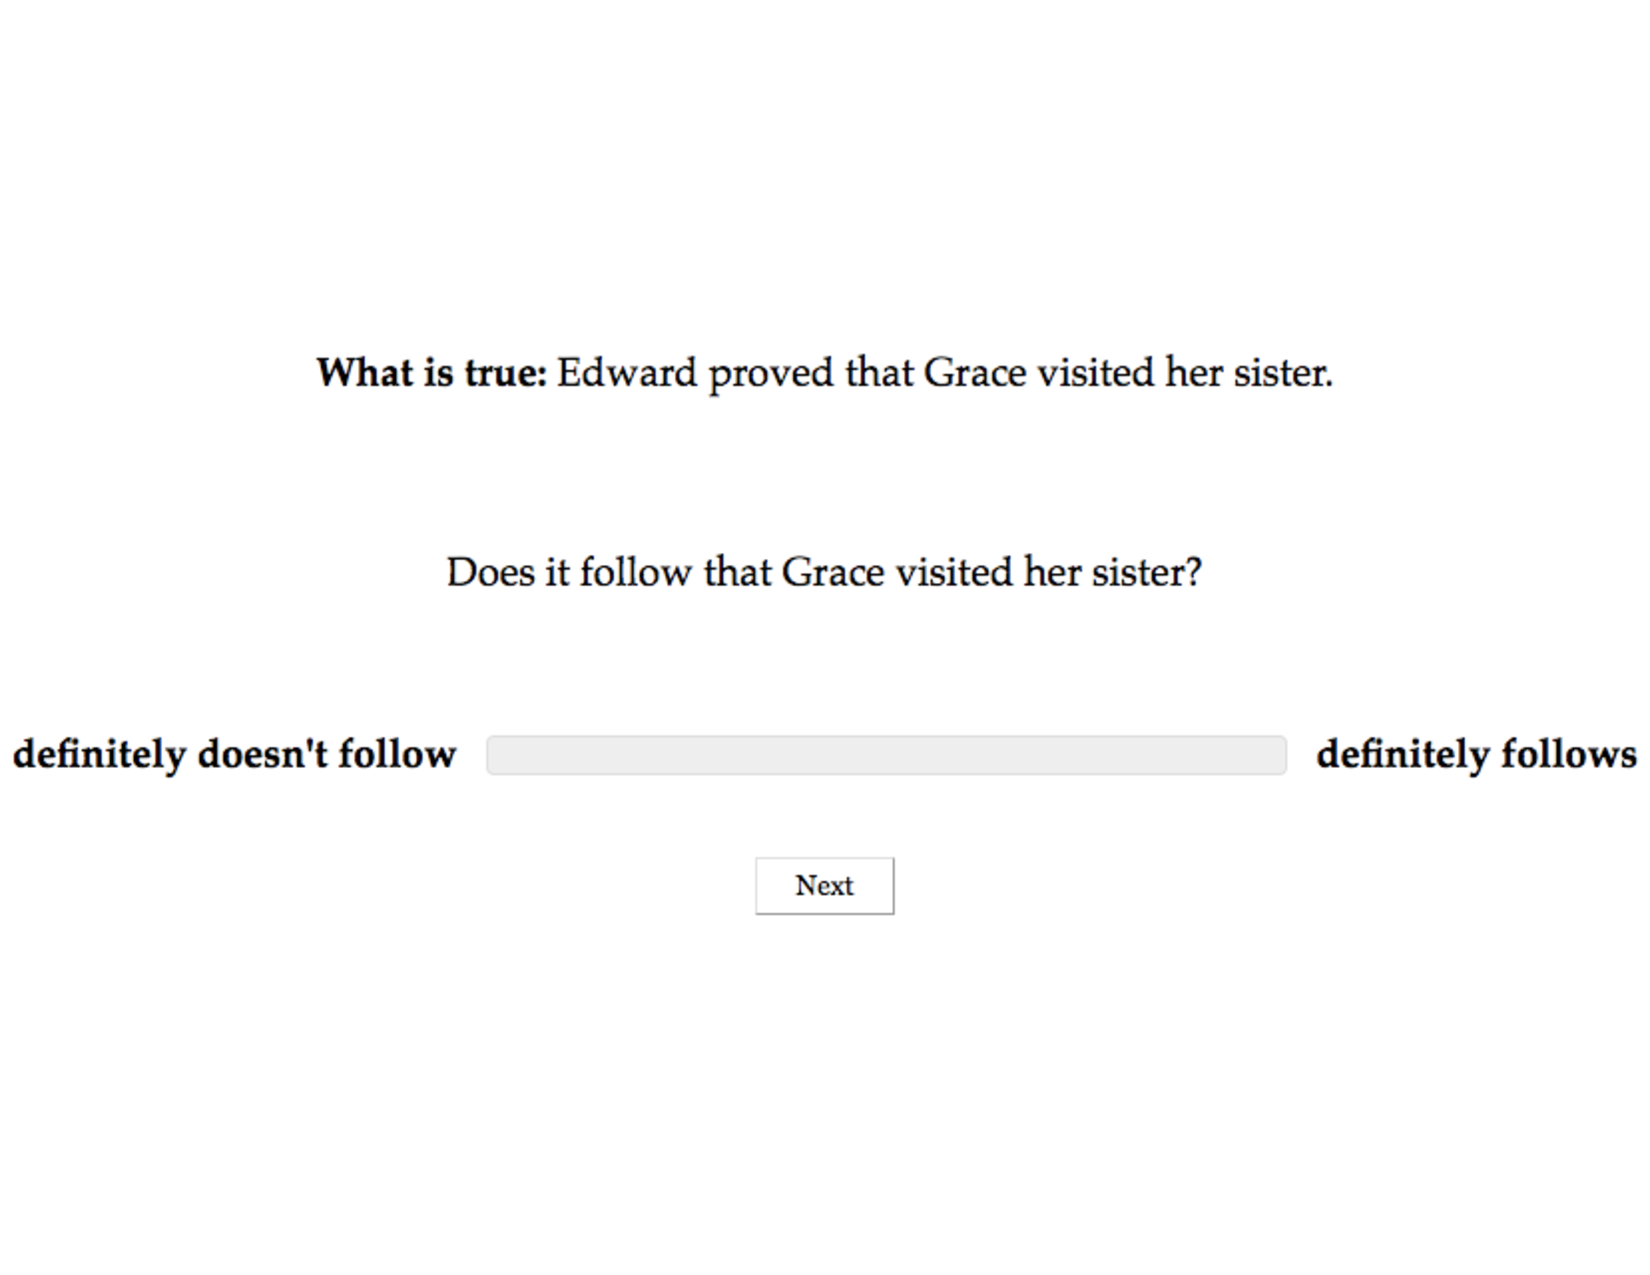
\includegraphics[width=13cm]{figures/inference-trial}}
\end{center}
\caption{A sample trial in Experiment 2a}\label{f-trial-exp3}
\end{figure}

To familiarize participants with the task, they first responded to the two familiarization stimuli in (\ref{train2}), where the inference tested was the inference to the CC. Participants who rated (\ref{train2}a) in the lower half of the sliding scale or (\ref{train2}b) in the upper half of the sliding scale were given an explanation for why their answer was wrong. Participants could only advance to the 28 stimuli if they gave a plausible rating to the two familiarization stimuli, that is, a rating in the upper half of the scale for (\ref{train2}a) and in the lower half for (\ref{train2}b).

\begin{exe}
\ex\label{train2}
\begin{xlist}
\ex {\bf What is true:} Drew is correct that Patty lives in Canada. 

\ex {\bf What is true}: Drew believes that Patty lives in Canada.
\end{xlist}
\end{exe}

After responding to the 28 stimuli, participants filled out a short, optional survey about their age, their gender, their native language(s) and, if English is their native language, whether they are a speaker of American English (as opposed to, e.g., Australian or Indian English). To encourage them to respond truthfully, participants were told that they would be paid no matter what answers they gave in the survey.

\paragraph{Data exclusion}

Prior to analysis, the data from 14 participants who did not self-identify as native speakers of American English were excluded. For the remaining 286 participants, we inspected their responses to the 8 control stimuli. The group mean for the four control stimuli in (\ref{control-good2}), for which the strength of the inference was expected to be at ceiling, was .94. The group mean for the four control stimuli in (\ref{control-bad2}), for which the strength of the inference was expected to be at floor, was .05. These group means suggest that, overall, participants attended to and understood the task. Importantly, the at-ceiling mean rating for the control stimuli with indisputably entailed content shows that the diagnostic can detect entailed content. The response means of 27 participants were more than 2 standard deviations below the group mean for the control stimuli in (\ref{control-good2}) or above the group mean for the control stimuli in (\ref{control-bad2}). Closer inspection revealed that these participants' responses to the control stimuli were systematically higher or lower, respectively, suggesting that these participants did not attend to the task or interpreted the task differently. The data from these 27 participants were also excluded. In this experiment, we did not identify any participants who always selected roughly the same point on the response scale. The results presented below are based on data from 259 participants (ages 19-69; median: 36; 132 female, 128 male). %; the group means were .96 for the control stimuli in (\ref{control-good2}) and .03 for the control stimuli in (\ref{control-bad2}).

\subsubsection{Results}

% prove is entailed, but be right is not, anything below it isn't either.

Figure \ref{f-veridicality-predicate} plots the mean inference ratings for the target stimuli by predicate, in increasing order from left to right, as well as for the non-entailing controls (abbreviated `non-ent.\ C') and the entailing controls (abbreviated `entailing C'). %As before, factive predicates are given in purple, optionally factive predicates in orange, veridical non-factive predicates in blue, and non-veridical non-factive predicates in gray. Participants' individual ratings are given by light gray dots. 
In line with impressionistic judgments reported in the literature, the mean inference ratings for most factive predicates as well as the veridical non-factive predicate {\em be right} are quite high, suggesting strong inferences to the truth of the CC. The mean inference ratings of the purportedly factive predicate {\em reveal} and of the purportedly veridical non-factive predicate {\em demonstrate} are lower, suggesting comparatively weaker inferences to the truth of the CC. 

% 1 acknowledge 0.905  0.0182  0.0161 
% 2 admit       0.907  0.0207  0.0177 
% 3 announce    0.809  0.0296  0.0296 
% 4 be_annoyed  0.924  0.0160  0.0151 
% 5 be_right    0.955  0.0116  0.0106 
% 6 confess     0.890  0.0209  0.0186 
% 7 confirm     0.943  0.0115  0.0109 
% 8 demonstrate 0.854  0.0266  0.0246 
% 9 discover    0.944  0.00936 0.00932
%10 entailing C 0.961  0.00443 0.00410
%11 establish   0.903  0.0205  0.0191 
%12 hear        0.498  0.0402  0.0412 
%13 inform      0.833  0.0285  0.0266 
%14 know        0.931  0.0155  0.0134 
%15 non-ent. C  0.0297 0.00404 0.00429
%16 pretend     0.116  0.0268  0.0290 
%17 prove       0.956  0.0109  0.0102 
%18 reveal      0.903  0.0195  0.0172 
%19 say         0.683  0.0366  0.0390 
%20 see         0.948  0.0114  0.0102 
%21 suggest     0.343  0.0354  0.0363 
%22 think       0.316  0.0342  0.0330

\begin{figure}[h!]
\centering

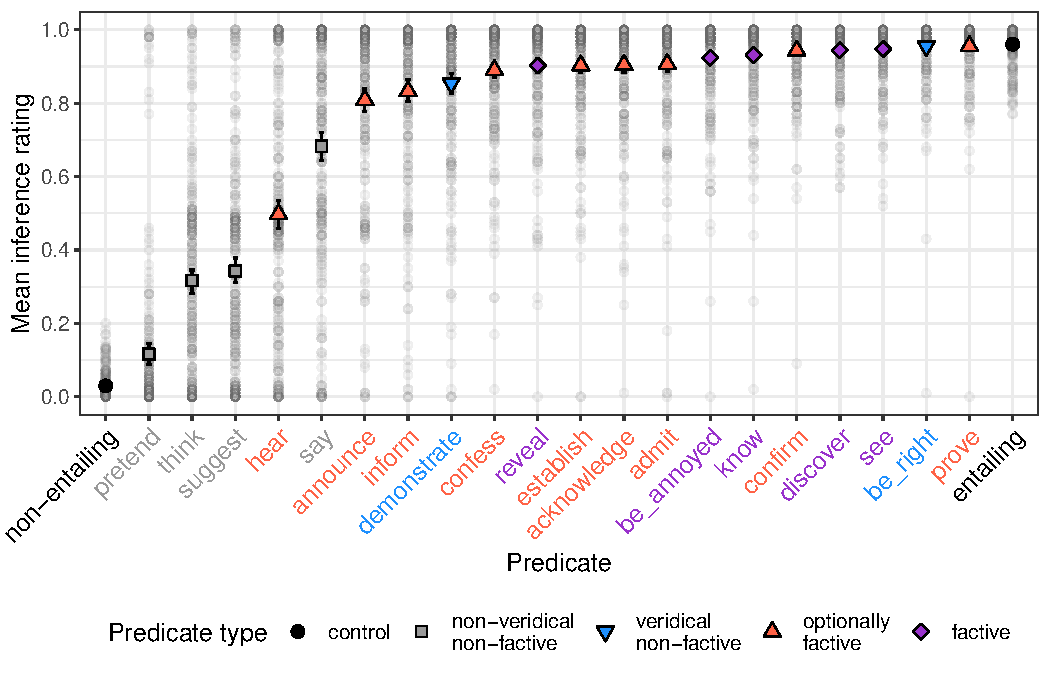
\includegraphics[width=.7\paperwidth]{../../results/4-veridicality3/graphs/means-inference-by-predicate-variability}

\caption{Mean inference rating by predicate, including the non-entailing controls (`non-ent.\ C') and the entailing controls (`entailing C'). Error bars indicate bootstrapped 95\% confidence intervals. Light gray dots indicate individual participants' ratings.} %Factive predicates are given in purple, veridical non-factive ones in blue, optionally factive ones in orange and non-veridical non-factive ones in gray.}
\label{f-veridicality-predicate}
\end{figure}

\jd{Describe model and update the following if necessary} In other words, only the inference ratings to the CC of {\em prove} are statistically indistinguishable from those of the controls with indisputably entailed content, suggesting that the CCs of the remaining 19 predicates are not entailed.

\subsubsection{Discussion}



\subsection{Experiment 2b: Categorical entailment ratings using inference diagnostic}

\subsubsection{Methods}

\paragraph{Participants} \jd{XXX} participants with U.S.\ IP addresses and at least 99\% of previous HITs approved were recruited on Amazon's Mechanical Turk platform They were paid \$\jd{XXX} for participating in the experiment.

\paragraph{Materials and procedure} The materials and procedure were identical to those of Exp.~2a, with the exception of the task: participants responded `yes' or `no' to the question of whether the CC follows from the true statement in which it was embedded. 

\paragraph{Data exclusion} Prior to analysis, we excluded the data from participants who did not self-identify as native speakers of American English. If a participant took an experiment more than once, we only analyzed the data from the first time they took the experiment \jd{how many?}. We also excluded the data from participants who gave a wrong rating to at least one control\jd{again, the problem of building in the zero-variability in the control conditions}: a rating was considered wrong if it was a `yes' rating on a non-entailing control or a `no' rating on an entailing control. The data from 341 participants (ages 18- 73; median: 38; 180 female, 161 male) entered the analysis below. 
    

\subsubsection{Results and discussion}

Figure \ref{fig:2bresults} shows the proportion of `yes' ratings on target trials by predicate, in increasing order from left to right, as well as on non-entailing control trials (abbreviated `non-ent.\ C') and entailing control trials (abbreviated `entailing C'). The findings of Exp.~2b are strikingly similar to those of Exp.~2a: the proportions of `yes' ratings are quite high for most factive predicates as well as the veridical non-factive predicate {\em be right} and the optionally factive predicate \emph{prove}, but the proportions for the purportedly factive predicate {\em reveal} and the purportedly veridical non-factive predicate {\em demonstrate} are lower. The order of predicates according to the categorical inference measure in  Exp.~2b is strikingly similar to that obtained via the continuous inference measure in Exp.~2a, as evidenced by the very high Spearman rank correlation of .996 (see Appendix \ref{a-binary} for a visualization).

The critical findings of Exp.~2a were replicated.  \jd{insert model info here once issue of exclusions settled} 
 
\begin{figure}[H]
\centering
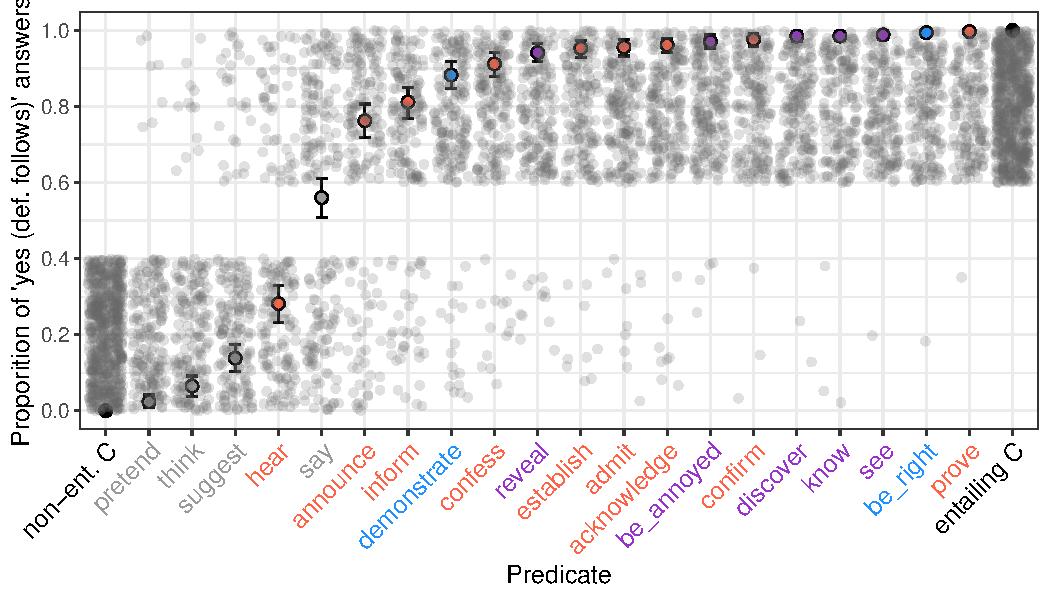
\includegraphics[width=.7\paperwidth]{../../results/7-veridicality3-binary/graphs/proportion-by-predicate-variability-individual}

\caption{Proportion of `yes' ratings by predicate. Error bars indicate 95\% bootstrapped confidence intervals. Jittered light gray dots indicate individual participants' ratings of `yes' (coded as 1) and `no' (coded as 0). }
\label{fig:2bresults}
\end{figure}


\subsection{Experiment 3a: Continuous entailment ratings using contradictoriness diagnostic}\label{s32}

This experiment investigated which of the CCs of the 20 clause-embedding predicates are entailed based on the contradictoriness diagnostic for entailment in (\ref{diag}b). Participants rated the contradictoriness of utterances of English sentences of the form {\em $\phi$ but not $\psi$}, where $\phi$ is an unembedded matrix sentence with a clause-embedding predicate and $\psi$ is its clausal complement, as in (\ref{announce3}):

\begin{exe}
\ex\label{announce3} Mary announced that she is pregnant, but she's not.
\end{exe}
Contextual factors may influence contradictoriness ratings: for instance, how contradictory an utterance of (\ref{announce3}) is assessed to be may depend on how old or how trustworthy Mary is (see, e.g., \citealt{schlenker10,demarneffe-etal2012}). To allow participants' ratings to reflect degrees of contradictoriness, we collected gradient contradictoriness ratings. We assume that when the content of $\phi$ entails the content of $\psi$, the contradictoriness of an utterance of the form {\em $\phi$ but not $\psi$} is not mitigated by contextual factors, and participants' contradictoriness ratings are at ceiling, that is, indistinguishable from contradictory control stimuli.

\subsubsection{Methods}

\paragraph{Participants} 300 participants with U.S.\ IP addresses and at least 99\% of previous HITs approved were recruited on Amazon's Mechanical Turk platform (ages: 18-72, median: 35; 137 female, 162 male, 1 other). They were paid \$0.75 for participating in the experiment.

\paragraph{Materials} In the target stimuli, the 400 predicate/clause combinations were combined with a random proper name subject and a {\em but-}clause that denied the truth of the CC. As shown in ({\ref{stims}), the target stimuli were presented to participants as utterances by named speakers. The proper names that realized the speakers, the subjects of the 20 predicates and the subjects of the complement clauses were all unique. The gender of the proper name subject of the predicate was distinct from the gender of the proper name in the complement clause, to ensure that the pronoun in the elliptical {\em but-}clause unambiguously referred to the individual referred to in the complement clause of the predicate.

\begin{exe}
\ex\label{stims}
\begin{xlist}
\ex {\bf Christopher:} {\em ``Melissa knows that Danny ate the last cupcake, but he didn't.''}
\ex {\bf Susan:} {\em ``Jerry pretended that Emma studied on Saturday morning, but she didn't.''}
\end{xlist}
\end{exe}

The experiment  included eight control stimuli that were used to assess whether participants were attending to the task and interpreted the task correctly, as well as to identify contradictoriness ratings for entailed content. (These stimuli were also presented to the participants as utterances by named speakers.) For the four control stimuli in (\ref{control-bad}), we expected contradictoriness ratings to be at ceiling because the first clause of each of these stimuli entails the negation of the second clause: in (\ref{control-bad}a), for instance, the content of {\em Madison laughed loudly} entails that Madison laughed, that is, the negation of {\em she didn't laugh}. As discussed above, we rely on the contradictoriness ratings for these control stimuli to identify entailments. By contrast, we expect the contradictoriness ratings for the four non-contradictory control stimuli in (\ref{control-good}) to be at floor, because the content of the second clause does not contradict the content of the first clause: for instance, in (\ref{control-good}a), the content that Vanessa is good at math does not entail the negation of the content that the speaker is not good at math. 

\begin{exe}

\ex\label{control-bad} Contradictory control stimuli
\begin{xlist}
\ex Madison laughed loudly and she didn't laugh.

\ex Dana has never smoked in her life and she stopped smoking recently.
\ex Hendrick's car is completely red and his car is not red.

\ex Sebastian lives in the USA and has never been to the USA.
\end{xlist}

\ex\label{control-good} Non-contradictory control stimuli
\begin{xlist}
\ex Vanessa is really good at math, but I'm not.
\ex Zack believes that I'm married, but I'm actually single.
\ex Tara wants me to cook for her and I'm a terrific cook.
\ex Frederick is both smarter and taller than I am.

\end{xlist}

\end{exe}

Each participant saw a random set of 28 stimuli: each set contained one target stimulus for each of the 20 predicates (each with a unique complement clause) and the same 8 control stimuli. Trial order was randomized.


\paragraph{Procedure.} Participants were told that they would read utterances made by a speaker and were asked to assess whether the speaker's utterance is contradictory. On each trial, participants read the speaker's utterance and then gave their response on a slider marked `definitely no' at one end (coded as 0) and `definitely yes' at the other (coded as 1), as shown in Figure \ref{f-trial-exp2}.

\begin{figure}[h!]
\begin{center}
\fbox{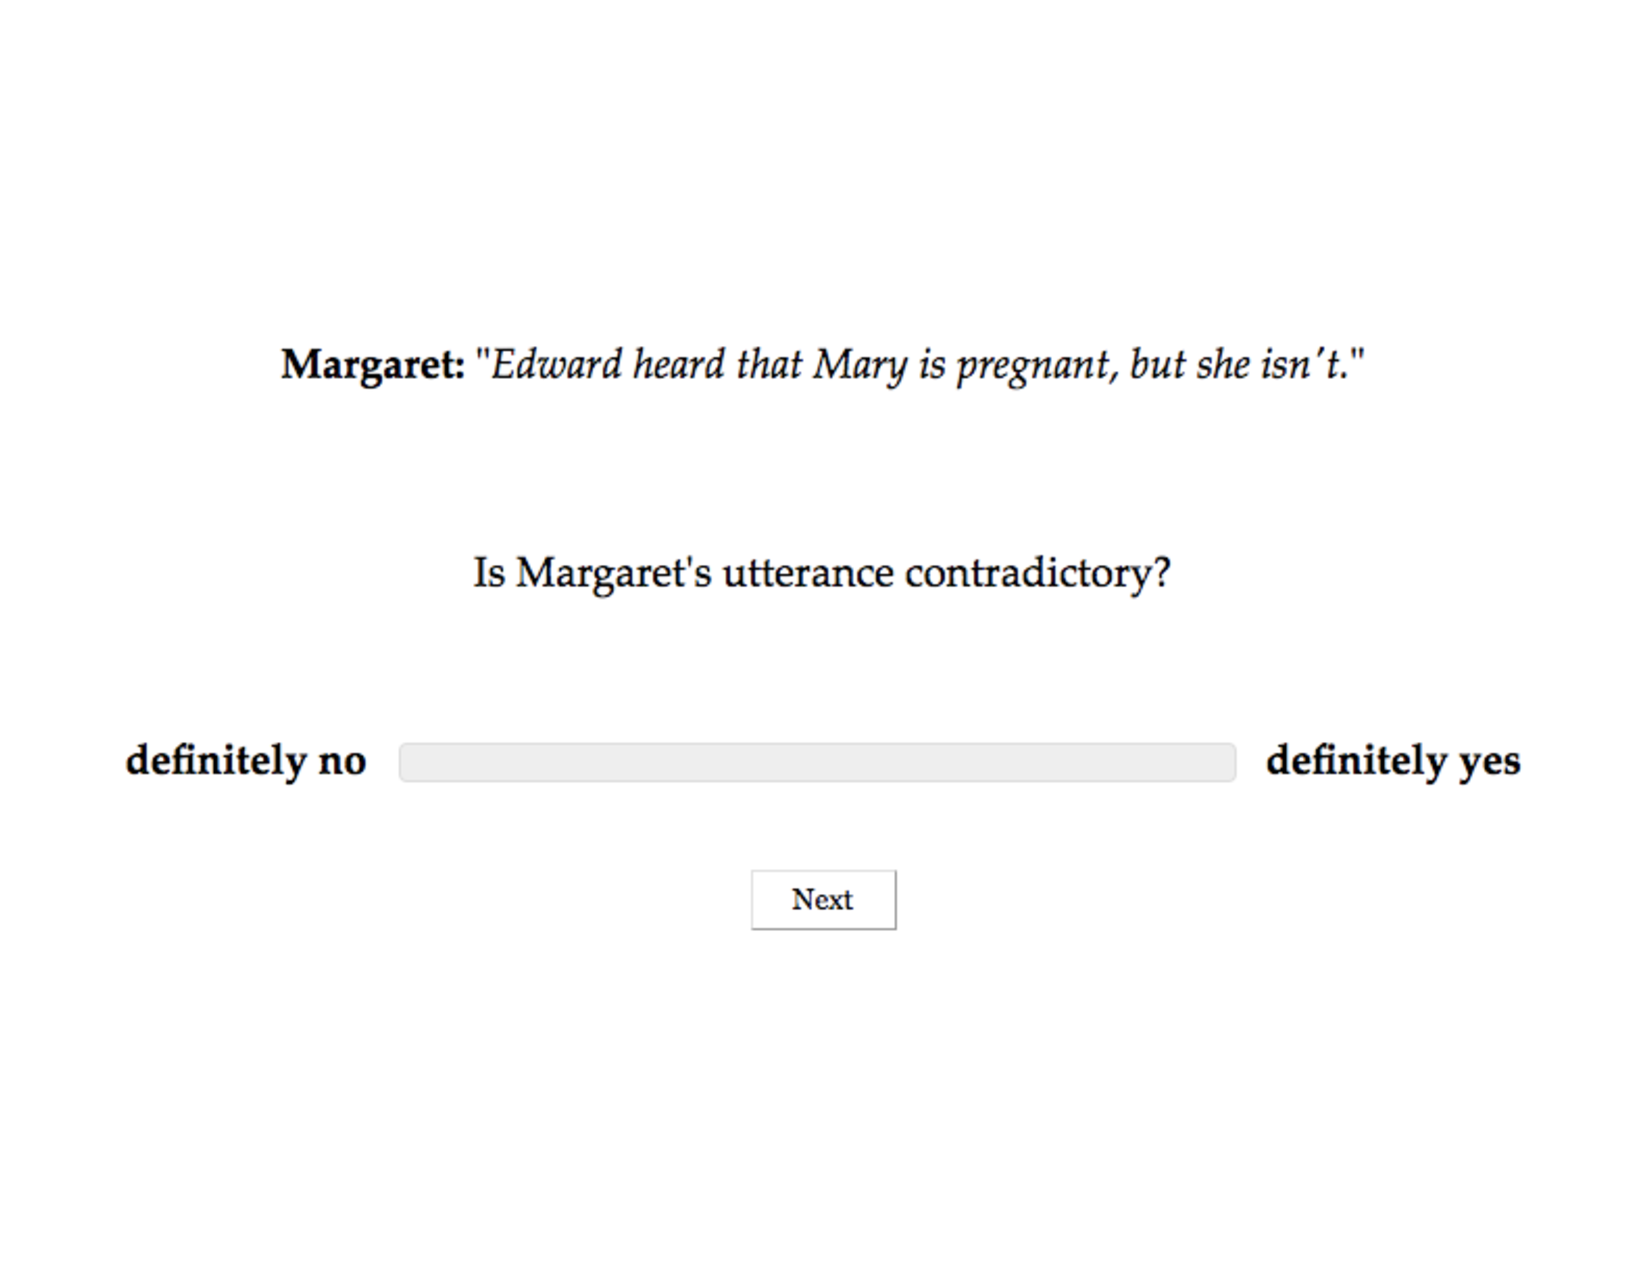
\includegraphics[width=13cm]{figures/contradictory-trial}}
\end{center}
\caption{A sample trial in Experiment 2b}\label{f-trial-exp2}
\end{figure}

To familiarize participants with the task, they first responded to the two familiarization stimuli in (\ref{train}): participants who rated (\ref{train}a) in the lower half of the scale or (\ref{train}b) in the upper half of the scale were given an explanation for why their answer was wrong. Participants could only advance to the 28 stimuli if they gave a plausible rating to the two training stimuli, that is, a rating in the upper half of the scale for (\ref{train}b) and a rating in the lower half for (\ref{train}b).

\begin{exe}
\ex\label{train}
\begin{xlist}
\ex Drew is aware that Patty lives in Canada, but she doesn't.

\ex Drew thinks that Patty lives in Canada, but she doesn't.
\end{xlist}
\end{exe}

After responding to the 28 stimuli, participants filled out a short, optional survey about their age, their gender, their native language(s) and, if English is their native language, whether they are a speaker of American English (as opposed to, e.g., Australian or Indian English). To encourage them to respond truthfully, participants were told that they would be paid no matter what answers they gave in the survey.

\paragraph{Data exclusion}

Prior to analysis, the data from 19 participants who did not self-identify as native speakers of American English were excluded. For the remaining 281 participants, we inspected their responses to the 8 control stimuli: as expected, the group mean rating for the non-contradictory control stimuli in (\ref{control-good}) was at floor (.08)\footnote{The mean contradictoriness rating of the non-contradictory control stimulus that was of the same form as the target stimuli, namely (\ref{control-good}b) {\em Zack believes that I'm married, but I'm actually single}, was higher, at .17, than the mean ratings of the remaining three non-contradictory control stimuli (means: .05 or .06) and identical to that of the target stimuli with {\em think}.}  and the group mean rating for the contradictory control stimuli in (\ref{control-bad}) was at ceiling (.94). This finding shows that, overall, participants attended to and understood the task. Importantly, the at-ceiling mean rating for the control stimuli with indisputably entailed content shows that the diagnostic can detect entailed content. The mean ratings of 18 participants were more than 2 standard deviations above the group mean for the non-contradictory control stimuli or below the group mean for the contradictory control stimuli. Closer inspection revealed that these participants' responses to the control stimuli were systematically higher or lower, suggesting that they did not attend to the task or interpreted the task differently. The data from these 18 participants were also excluded. In this experiment, we did not identify any participants who always selected roughly the same point on the response scale. The results presented below are based on data from 263 participants (ages 18-72; median: 36; 126 female, 136 male, 1 other).

\subsubsection{Results}

% ZOIB model: be_right is significantly less contradictory than contradictory controls

Figure \ref{f-veridicality-predicate2} plots the mean contradictoriness ratings for the target stimuli by predicate, in increasing order from left to right, as well as for the non-contradictory controls (abbreviated `non-contrd.\ C')  and  the contradictory controls (`contradictory C'). As before, factive predicates are given in purple, optionally factive predicates in orange, veridical non-factive predicates in blue, and non-veridical non-factive predicates in gray. Participants' individual ratings are given by light gray dots. In line with impressionistic judgments reported in the literature, the mean inference ratings for the factive and veridical non-factive predicates are among the highest, and those of the non-factive predicates are among the lowest. However, except possibly for {\em be right}, none of the mean contradictoriness ratings are at ceiling.

%   verb              Mean
%   <chr>            <dbl>
% 1 acknowledge     0.672 
% 2 admit           0.711 
% 3 announce        0.448 
% 4 be_annoyed      0.640 
% 5 be_right        0.941 
% 6 confess         0.669 
% 7 confirm         0.767 
% 8 contradictory C 0.960 
% 9 demonstrate     0.720 
%10 discover        0.789 
%11 establish       0.721 
%12 hear            0.238 
%13 inform          0.472 
%14 know            0.838 
%15 non-contrd. C   0.0587
%16 pretend         0.217 
%17 prove           0.858 
%18 reveal          0.634 
%19 say             0.363 
%20 see             0.819 
%21 suggest         0.257 
%22 think           0.171 

\begin{figure}[h!]
\centering

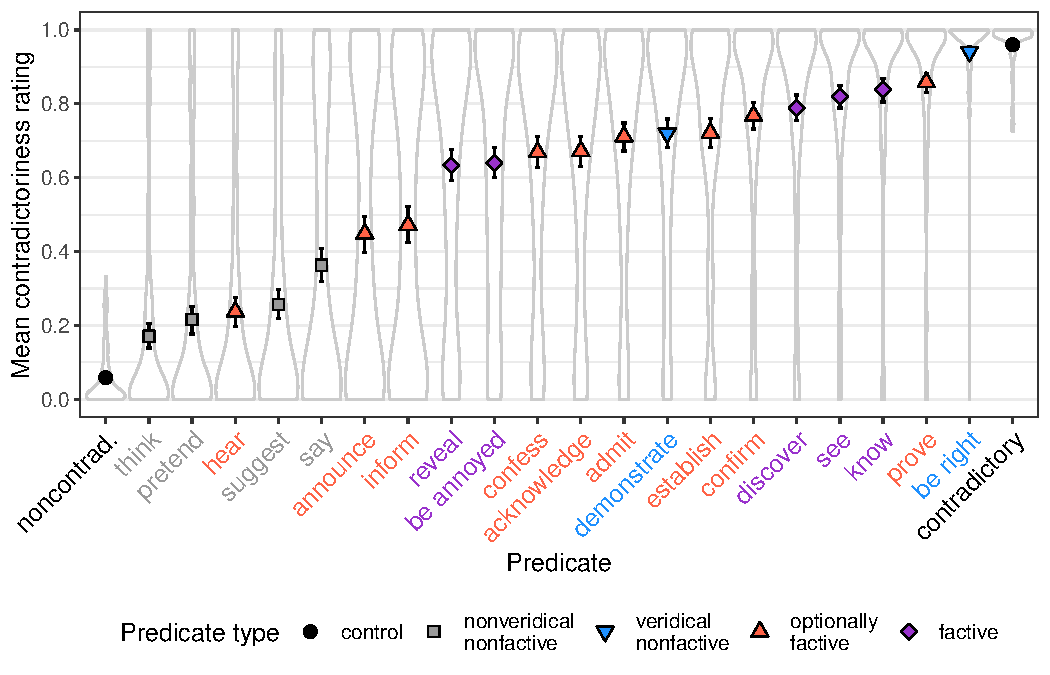
\includegraphics[width=.7\paperwidth]{../../results/2-veridicality2/graphs/means-contradictoriness-by-predicate-variability}

\caption{Mean contradictoriness rating by predicate, collapsing over complements, including the non-contradictory controls (`non-contrd.\ C') and the contradictory controls (`contradictory C'). Error bars indicate bootstrapped 95\% confidence intervals. Light gray dots indicate individual participants' ratings. Factive predicates are given in purple, veridical non-factive ones in blue, optionally factive ones in orange and non-veridical non-factive ones in gray.}
\label{f-veridicality-predicate2}
\end{figure}

{\bf Describe models} In other words, none of the contradictoriness ratings for the CCs are statistically indistinguishable from those of the controls with indisputably entailed content, suggesting that the CCs of all 20 predicates are not entailed.

\subsection{Experiment 3b: Categorical entailment ratings using contradictoriness diagnostic}
\label{s32}

\subsubsection{Methods}

\paragraph{Participants} \jd{XXX} participants with U.S.\ IP addresses and at least 99\% of previous HITs approved were recruited on Amazon's Mechanical Turk platform They were paid \$\jd{XXX} for participating in the experiment.

\paragraph{Materials and procedure} The materials and procedure were identical to those of Exp.~3a, with the exception of the task: participants responded `yes' or `no' to the question of whether the speaker's utterance is contradictory. 

\paragraph{Data exclusion} Prior to analysis, we excluded the data from participants who did not self-identify as native speakers of American English. If a participant took an experiment more than once, we only analyzed the data from the first time they took the experiment \jd{how many?}. We also excluded the data from participants who gave a wrong rating to at least one control\jd{again, the problem of building in the zero-variability in the control conditions}: a rating was considered wrong if it was a `yes' rating on a non-contradictory control or a `no' rating on a contradictory control. The data from 302 participants (ages 18- 73; median: 37; 150 female, 152 male) entered the analysis below. 
    


\subsubsection{Results}

\jd{add description}

\begin{figure}
\centering
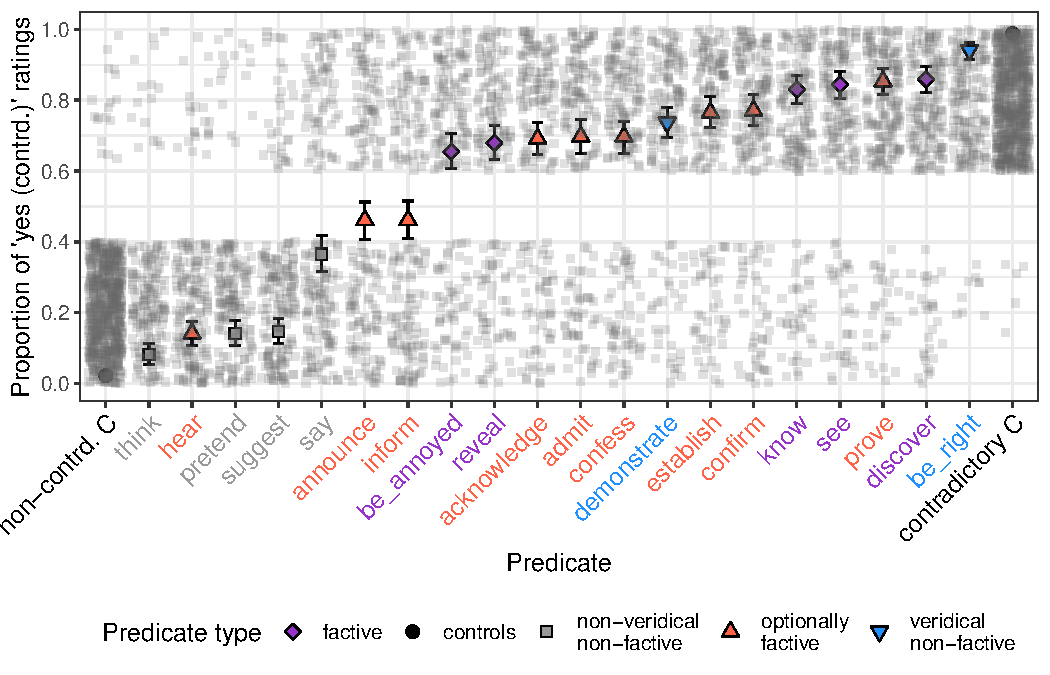
\includegraphics[width=.7\paperwidth]{../../results/6-veridicality2-binary/graphs/proportion-by-predicate-variability-individual}
\caption{Proportion of `yes' ratings by predicate. Error bars indicate 95\% bootstrapped confidence intervals. Jittered light gray dots indicate individual participants' ratings of `yes' (coded as 1) and `no' (coded as 0). }
\label{f-binary}
\end{figure}

\subsection{Discussion}\label{s33}

In Exps.~2, we applied two standard diagnostics for entailment to the CCs of 20 clause-embedding predicates, with the goal of identifying predicates whose CC is entailed content. To assess whether the CC of a particular predicate is entailed, we compared the inference ratings (Exp.~2a) and the contradictoriness ratings (Exp.~3a) for the CCs to the ratings for control stimuli with indisputably entailed content: we assumed that the CC of a predicate is entailed if the ratings for that CC are statistically indistinguishable from these control stimuli, and not entailed if the ratings for that CC are significantly lower. Given these assumptions, we found that the CC of {\em prove} is entailed according to the inference diagnostic and that the CC of none of the 20 predicates is entailed according to the contradictoriness diagnostic. 

Our way of identifying entailed CCs, namely by comparing them to indisputably entailed content, was motivated by the standard definition of entailment. One can, of course, ask whether there might be better ways of identifying entailed CCs. For instance, one might consider those CCs entailed whose mean inference or contradictoriness ratings are at least as high as those of {\em demonstrate}, that is .85 or .72, respectively: this would mean that the CCs of all of the predicates typically taken to be factive or veridical non-factive are entailed, as well as the CCs of some optionally factive predicates. There is, however, no principled reason why the ratings for the CC of {\em demonstrate} should be the threshold for entailment. One could also pick an arbitrary mean inference or mean contradictoriness rating, say .8, and categorize CCs with mean ratings of at least .8 as entailed, and CCs with mean ratings below .8 as not entailed. Of course, this way of identifying entailed CCs is also not principled. After all, one could just as well pick a threshold of .85 or .75, with the result that the CCs of different predicates would be considered entailed: for instance, on the contradictoriness diagnostic, the CC of {\em discover} (mean: .79) would not count as entailed with a threshold of .8, but would with one of .75, and the CC of {\em know} (mean: .84) would count as entailed with a threshold of .8, but not with one  of .85. Furthermore, neither of these alternative ways of identifying entailed CCs are compatible with the standard definition of entailment because, under both, one would need to allow for CCs to count as entailed even though they received significantly lower ratings than indisputably entailed content.

One might also wonder whether a different entailment diagnostic might result in the CCs of more clause-embedding predicates being classified as entailed. For instance, one might wonder whether the gradient response scale on which participants responded in Exps.~2 contributed to so few CCs being classified as entailed and whether the finding would be different if participants had been asked to decide in a two-alternative forced choice task whether the content follows from a true statement, on the inference diagnostic, or whether the speaker's utterance is contradictory, on the contradictoriness diagnostic. To assess this possibility, we ran two follow-up experiments that were identical to Exps.~2 except that we used a two-alternative forced choice task, with `yes' (coded as 1) or `no' (coded as 0) as the response options (see Appendix \ref{a-binary} for details). We refer to these two experiments as Exp.~2a$'$ and Exp.~3a$'$. The two plots in Figure \ref{f-binary} show the proportion of `yes' ratings on the two diagnostics by predicate, again in increasing order from left to right, as well as the ratings for two types of control stimuli. Jittered light gray dots indicate individual participants' ratings. The findings of Exps.~2$'$ are strikingly similar to those of Exps.~2: on the inference diagnostic (panel a), the proportions of `yes' ratings are quite high for most factive predicates as well as the veridical non-factive predicate {\em be right}, but the proportions for the purportedly factive predicate {\em reveal} and the purportedly veridical non-factive predicate {\em demonstrate} are lower; on the contradictoriness diagnostic (panel b), the proportion of `yes' ratings for {\em be right} are quite high, but those of the factive predicates and of the other veridical non-factive predicate are not. The Spearman rank correlations for the two pairs of experiments are very high, providing further evidence for the similarities between the findings: .996 for the two experiments that used the inference diagnostic (Exps.~2a and 2a$'$) and .985 for the two experiments that used the contradictoriness diagnostic (Exps.~2b and 2b$'$); see Appendix \ref{a-binary} for figures.

\begin{figure}[H]
\centering

\begin{subfigure}{1\textwidth}
\centering
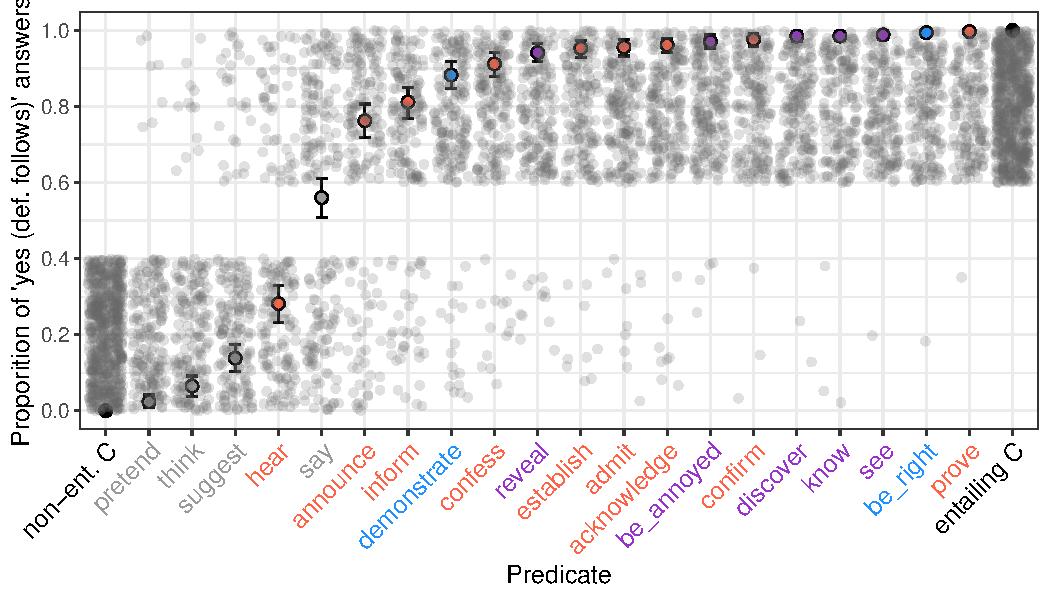
\includegraphics[width=.7\paperwidth]{../../results/7-veridicality3-binary/graphs/proportion-by-predicate-variability-individual}
\caption{Inference diagnostic for entailment.}
\end{subfigure}

\begin{subfigure}{1\textwidth}
\centering
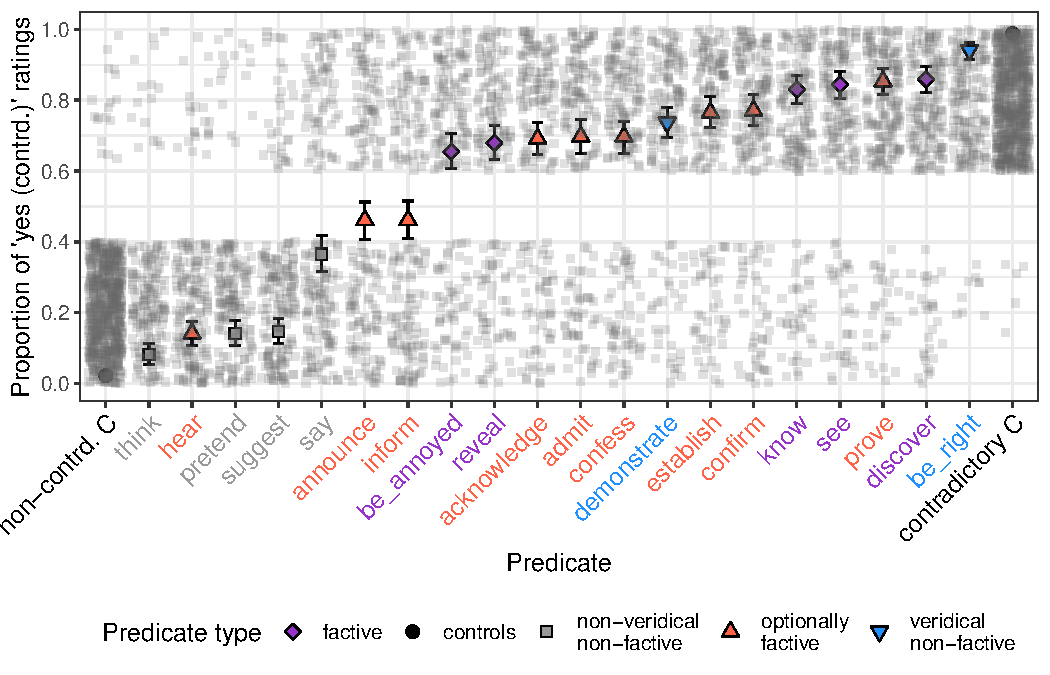
\includegraphics[width=.7\paperwidth]{../../results/6-veridicality2-binary/graphs/proportion-by-predicate-variability-individual}
\caption{Contradictoriness diagnostic for entailment}
\end{subfigure} 

\caption{Proportion of `yes' ratings by predicate, with 95\% bootstrapped confidence intervals, collapsing over complement clauses. Factive predicates are given in purple, veridical non-factive ones in blue, non-veridical non-factive ones in gray and optionally factive ones in orange. Jittered light gray dots indicate individual participants' ratings of `yes' (coded as 1) and `no' (coded as 0). }
\label{f-binary}
\end{figure}

To identify predicates whose CCs are entailed on Exps.~2$'$, we ideally want to compare the ratings for the CCs to those of the controls with indisputably entailed content, as in Exps.~2. However, in contrast to the CCs of the 20 predicates, to which participants gave `no' ratings (indicating no entailment), there are no `no' ratings for the relevant controls: on the inference diagnostic (panel a) none of the 341 participants whose data are plotted responded `no' to any of the four entailing control stimuli (1,364 data points) and, on the contradictoriness diagnostic (panel b), none of the 302 participants whose data are plotted responded `no' to any of the four contradictory control stimuli (1,208 data points). This lack of variability in the ratings of the relevant control stimuli means that we cannot use the control conditions as reference levels. {\bf Explain why}

Because we were not able to use the controls with indisputably entailed content to identify entailed CCs, we made do by assuming that the CCs of the predicates that received the highest proportion of `yes' ratings are entailed and used those predicates as reference levels: this was {\em prove} with 340 out of 341 `yes' ratings on the inference diagnostic and {\em be right} with 291 out of 302 `yes' ratings on the contradictoriness diagnostic. {\bf Discuss models} In other words, on the inference diagnostic, the ratings for {\em be right, discover, know} and {\em see} are indistinguishable from those of {\em prove} and, on the contradictoriness diagnostic, the ratings for none of the predicates are indistinguishable from those of {\em be right}. Given the assumption that the CCs of {\em prove} and {\em be right} are entailed content, the findings of the inference diagnostic follow-up experiment suggest that the CCs of {\em be right, discover, know} and {\em see} are entailed. In sum, we have only found partial confirmation for the hypothesis that it was due to the gradient response scale of Exps.~2 that hardly any of the 20 clause-embedding predicates were found to have entailed CCs: the CCs of more clause-embedding predicates were classified as entailed by Exp.~2a$'$ than by Exp.~2a, but not by Exp.~3a$'$ compared to Exp.~3a (recall that the CC of {\em be right} is entailed merely by assumption).\footnote{To be able to compare the findings from the two experiments, we fit a model to the Exp.~2a data with {\em prove} as the reference level. {\bf Describe model} In other words, on that model the ratings for all predicates are lower than those of {\em prove}.} 

This means that we still cannot conclude with any confidence that the CC of any of the 20 predicates we investigated is entailed. The CC of {\em prove} is entailed according to Exp.~2a, but not according to Exps.~2b or 2b$'$. (We assumed that it was entailed in Exp.~2a$'$.) And although Exp.~2a$'$ suggested that the CCs of {\em be right, discover, know} and {\em see} are entailed, we have no reason to assume that Exp.~2a$'$ is better at diagnosing entailment than Exps.~2a, 2b and 2b$'$, all of which provided evidence that the CCs of these predicates are not entailed. It is possible, for instance, that Exp.~2a$'$ resulted in more entailed CCs because participants chose `yes' even if they would have given an inference rating below ceiling on the gradient scale of Exp.~2a. It is also not clear that the inference diagnostic is more suitable to diagnosing entailment than the contradictoriness diagnostic: it is possible that even non-entailed content receives high inference ratings and that participants find it easier to identify non-entailed CCs when judging a potentially contradictory utterance. We therefore conclude that we do not have conclusive evidence that the CC of any of the 20 predicates we investigated is entailed.

This conclusion, we argue, is not due to the inference or the contradictoriness diagnostics not being able to diagnose entailed content: after all, control stimuli with indisputably entailed content received at-ceiling ratings in all four experiments.\footnote{\citet[329]{demarneffe-etal2012} suggested that veridicality ratings are influenced by pragmatic reasoning. We agree with this possibility but consider it unlikely that pragmatic reasoning would only influence participants' ratings on the target stimuli, to the exclusion of the control stimuli.} Further evidence for our conclusion comes from the MegaVeridicality dataset, introduced in section \ref{s22}, which also contains entailment ratings for the CCs of the 517 English clause-embedding predicates; these ratings were collected for stimuli that combined these predicates with arguments with low lexical content, as shown in (\ref{wr-stim-ent}) for the predicate {\em know}. To assess entailment, participants were asked to respond to the question {\em Did that thing happen?}; the response options were `yes', `maybe or maybe not' and `no'. 

\begin{exe}
\ex\label{wr-stim-ent} Somebody knew that a particular thing happened.
\end{exe}

Each of the 517 predicates in the MegaVeridicality dataset received between 9 and 20 entailment ratings (mean: 10) from 159 participants. To plot the ratings, we coded a `yes' response as 1, a `maybe or maybe not' response as 0 and a `no' response as -1. Figure \ref{f-white-rawlins-ent} plots the mean entailment ratings for the 517 predicates in the MegaVeridicality dataset, with x-axis labels for 19 of the 20 predicates that we investigated.\footnote{The x-axis labels for the following predicates overlap: {\em acknowledge/announce/admit/confess/demonstrate} and {\em inform/know}.} There are 97 clause-embedding predicates that only received `yes' ratings, including 3 of the factive predicates we investigated, namely {\em reveal, know} and {\em be annoyed}; this finding is compatible with the assumption that the CCs of these predicates are entailed. 

\begin{figure}[H]
\centering
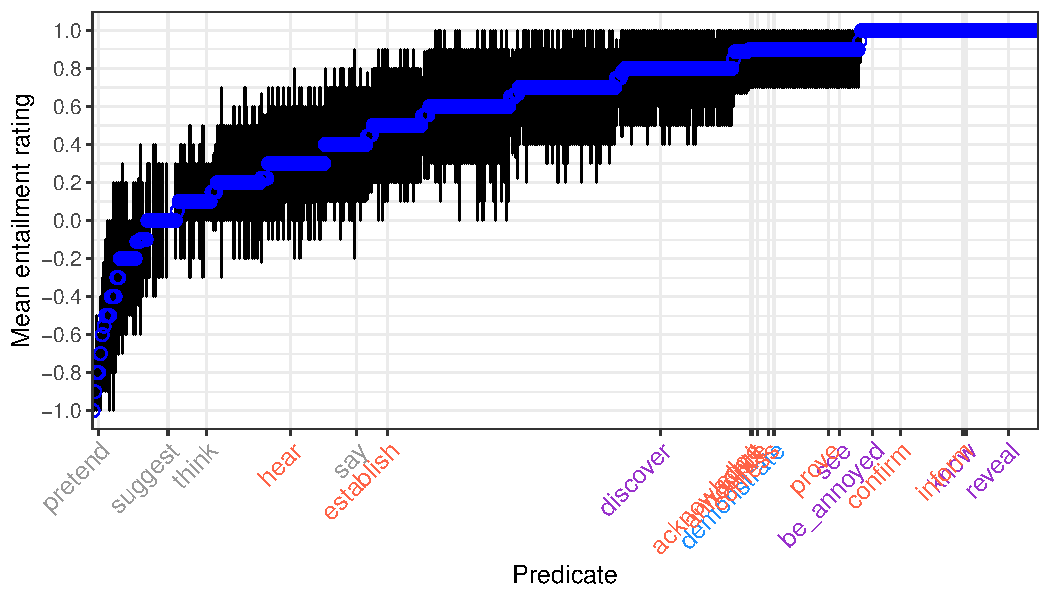
\includegraphics[width=.75\paperwidth]{../../white-rawlins-data/graphs/means-entailment-by-predicate}

\caption{Mean entailment rating in blue, by predicate, with 95\% bootstrapped confidence intervals, for the 517 predicates in MegaVeridicality dataset. X-axis labels for 19 of the 20 predicates featured in our Exps.~1 and 2: factive predicates in purple, the veridical non-factive one in blue, non-veridical non-factive ones in gray and optionally factive ones in orange.}
\label{f-white-rawlins-ent}
\end{figure}

However, as with our Exps.~2 and 2$'$, not all of the factive and veridical non-factive predicates we investigated received only `yes' ratings: the ratings for the purportedly factive predicates {\em see} and {\em discover} and for the purportedly veridical non-factive predicate {\em demonstrate} were not at ceiling, suggesting that their CCs are not entailed.\footnote{\label{mv}\citet{white-rawlins-nels2018} came to a different conclusion because they assumed that the CC of a predicate is entailed if and only if the majority of the responses for a predicate was `yes'. According to this linking function, the CCs of 376 of the 517 predicates in the MegaVeridicality dataset are entailed. We do not adopt this linking function because it is incompatible with the standard definition of entailment: for instance, given this linking function, {\em tweet} is a veridical predicate because 11 of the 20 participants responded `yes', despite the fact that the remaining 9 participants responded `maybe or maybe not'.} Furthermore, it is not clear that the CCs of the 97  predicates that only received `yes' ratings are entailed: this set of 97 predicates includes {\em inform} (see the discussion in section \ref{s1}) as well as the communication predicates {\em bitch} and {\em howl}, whose CCs are not entailed. For instance, it does not follow from the naturally occurring example with {\em bitch} in (\ref{bitch}) that the Democratic party hates all the Jews.

\begin{exe}
\ex\label{bitch} Rambling to reporters in the Oval Office, Trump bitched that the Democratic party clearly hates all the Jews because of all the support reps Rashida Tlaib and Ilhan Omar received after he strong armed the Israelis into barring them from visiting the country as members of Congress.\footnote{\url{https://www.wonkette.com/08-21-2019}}
\end{exe}
In sum, even though the MegaVeridicality database used a different entailment diagnostic and different response options than our experiments, it supports our conclusion that, of the 20 clause-embedding predicates we investigated, fewer than expected have entailed CCs. 
 
\subsection{Do projectivity and entailment jointly identify a class of factive predicates?}\label{s34}

As discussed in section \ref{s1}, a predicate is factive on the second definition if and only if its CC is presupposed and entailed. With data on projectivity and entailment in hand, we now return to the question of whether these two properties jointly distinguish a class of factive predicates from optionally factive and non-factive ones. We first consider the five purportedly factive predicates we investigated, namely {\em be annoyed, discover, know, reveal} and {\em see}. Regarding projectivity, Exp.~1a showed that the CC of each of these predicates is quite highly projective, in support of their categorization. Regarding entailment, however, Exps.~2 provided little empirical support for the assumption that the CCs of these predicates is entailed: although Exp.~2a$'$ provided support that the CCs of {\em discover, know} and {\em see} are entailed, Exps.~2a, 2b and 2b$'$ provided evidence that the CCs of none of the five are entailed. Thus, projectivity and entailment do not jointly identify these five predicates as factive.

Is there a different class of predicates that projectivity and entailment jointly identify as factive? One might consider the set of predicates consisting of {\em be annoyed, know, see, inform} and {\em discover}: regarding projectivity,  the CCs of each of these predicates are the most projective of the 20 predicates investigated. A problem, however, with assuming that this set of predicates is factive according to the second definition is that one would need to disregard the evidence from Exps.~2a, 2b and 2b$'$ that the CCs of these predicates are not entailed, even if Exp.~3a$'$ provided evidence for entailment for {\em know, see} and {\em discover}. Another set one might consider consists of {\em  prove, be right, discover, know} and {\em see}: regarding projectivity, the CCs of each of these predicates are projective, albeit only very weakly for some; regarding entailment, the CCs of each of these predicates were identified as entailed by at least one of Exps.~2 or 2$'$. One problem with assuming that this set of predicates is factive according to the second definition is that one would, again, need to disregard the evidence from Exps.~2 and 2$'$ that the CCs of these predicates are not entailed. Another problem is that this set of predicates does not form a natural class, given how much the CCs of these predicates differ in projectivity: for instance, assuming that these five predicates are factive would not be helpful in developing a theory of presupposition projection. We conclude that the second definition of factive predicates is no more successful than the first in distinguishing factive predicates from optionally factive and non-factive ones.\footnote{\citet{white-rawlins-nels2018}, who assumed the second definition of factive predicates, identified 199 factive predicates in the MegaVeridicality database. However,  this finding is due to the authors assuming that a majority of `yes' responses for a predicate means that the CC is entailed (for positive matrix sentences) or presupposed (for sentences embedded under negation or in a question). As discussed in footnote \ref{mv}, the linking function for entailed CCs is not compatible with the standard definition of entailment. For presupposed CCs, it is not clear that a majority of `yes' responses is motivated as a threshold for projection; see the discussion in section \ref{s22}.} 

\section{Discussion}\label{s4}

The question addressed in this paper is: Which predicates are factive? Despite the central role that the distinction between factive and non-factive predicates has played in linguistic theorizing, different answers have been given to this question because, as noted in section \ref{s1}, there is disagreement about how to define factive predicates, uncertainty about whether projection categorically distinguishes factive predicates from optionally factive and non-factive ones, and disagreement about which clause-embedding predicates have entailed CCs. In sections \ref{s2} and \ref{s3}, we presented the findings of experiments designed to investigate which predicates are factive based on  two definitions of factive predicates. Our experiments in section \ref{s2} investigated the first definition, according to which a predicate is factive if and only if its CC is presupposed: we found that projection alone does not categorically distinguish factive predicates from optionally factive and non-factive ones and, furthermore, that the CCs of all of the predicates we investigated are at least mildly projective. In section \ref{s3}, we investigated the second definition, according to which a predicate is factive if and only if its CC is both presupposed and entailed: our experiments did not provide conclusive evidence that the CCs of any of the 20 predicates we investigated are entailed and so we concluded that the second definition also does not identify a class of factive predicates. We are therefore led to the conclusion that, at present, there is no empirical evidence for a class of factive predicates that is categorically distinguished from optionally factive and non-factive ones by two properties of the CC, namely projection and entailment. 

This does not, of course, mean that no empirical evidence for a class of factive predicates could ever be provided. One might, for instance, maintain the second definition of factive predicates and explore other ways of diagnosing entailed CCs. As discussed in \citealt{demarneffe-etal2012} and \citealt{pavlick-kwiatkowski2019}, participants' veridicality ratings appear to be influenced by a variety of pragmatic factors; it is an intriguing question for future research whether one can sufficiently control these pragmatic factors to elicit purely semantic judgments about veridicality to support claims about entailment. Another option is to define factive predicates differently, for instance on the basis of some syntactic property or as predicates for which the majority of participants judge the CC to be projective and entailed (see, e.g., \citealt{white-rawlins-nels2018}). Such definitions will have to be assessed by the explanatory power of the resulting categorizations of clause-embedding predicates for the theoretical phenomenon under investigation. 

One area in which the distinction between factive and non-factive predicates has played a major role is research on projective content. Formal analyses of the projection of the CC of clause-embedding predicates are generally limited to the CCs of factive predicates: the explanandum is assumed to be that the CCs of factive predicates, but not those of optionally factive or non-factive ones, are presuppositions, which may project. On some analyses (e.g., \citealt{heim83,vds92}), factive predicates lexically specify that the CC is required to be entailed by or satisfied in the relevant context; optionally factive and non-factive predicates do not carry such a lexical specification. On other analyses (e.g., \citealt{abrusan2011,abrusan2016,romoli2015,best-question}), projection of the CC is derived from the CC being entailed content that is backgrounded; non-entailed CCs of optionally factive and non-factive predicates are again outside of the scope of these analyses. It is within the context of these formal analyses that we were led to investigate which predicates are factive: we wanted to understand which predicates these analyses apply to. Our conclusion that, at present, there is no empirical evidence for a class of factive predicates is unnerving because it means that it is not clear which predicates these analyses apply to.

Even though our investigation has not yielded a class of factive predicates, it has revealed that the CCs of more clause-embedding predicates than previously assumed are projective, albeit some are only mildly so. This finding means that research on projective content has a much broader empirical scope than previously assumed. Given that research on projective content has focused almost entirely on the the CCs of factive predicates, to the exclusion of the CCs of optionally factive and non-factive ones, our finding means that we are now tasked with investigating and formally analyzing the projectivity of the CCs of a much broader set of clause-embedding predicates than before. For instance, research on projective content has identified a number of factors that influence the projectivity of utterance content, including context, lexical content, prior content probability, at-issueness, information structure and the perceived degree of reliability and trustworthiness of the attitude holder (e.g., \citealt{gazdar79a,gazdar79b,beaver-belly,schlenker10,brst-salt10,best-question,abrusan2011,abrusan2016,anand-hacquard2014,cummins-rohde2015,djaerv-bacovcin-salt27,tonhauser-salt26,tonhauser-guarani-variability,tbd-variability,tonhauser-etal-sub23}). An exciting question for future research is whether these factors are implicated in the projectivity of the CCs of all clause-embedding predicates, or only particular subsets. 

On the theoretical side, our finding that the CCs of more clause-embedding predicates than previously assumed are projective calls for the development of formal analyses of the projectivity of these CCs. One approach to predicting the projectivity of the CCs of optionally factive and non-factive predicates has been to assume that such predicates are ambiguous: \citet{spector-egre2015}, for instance, proposed (p.1736) that predicates like {\em tell, predict} and {\em announce}  have a factive lexical entry on which the CC is entailed and presupposed and a non-factive one on which it is not. The findings of our Exps.~1 point to some difficulties for this approach, given that the CC of all 20 predicates we investigated is at least mildly projective. First, this approach requires the assumption of widespread ambiguity among clause-embedding predicates. Second, it is not clear which predicates would only have a factive or only a non-factive lexical entry, and which ones would be ambiguous. And, finally, the approach cannot account for the observed by-predicate projection variability: for instance, the assumption that both {\em discover} and {\em announce} have a factive and a non-factive lexical entry does not predict that the CC of {\em discover} more projective than the CC of {\em announce}.

We hypothesize that more fine-grained distinctions among the lexical meanings of clause-embedding predicates than the distinction between factive and non-factive predicates (or the three-way distinction between factive, optionally factive and non-factive predicates) matter for predicting speaker commitment to the CC, both in affirmative matrix clauses and under entailment-canceling operators. More specifically, we hypothesize that the CCs of classes of predicates that share lexical meanings and discourse uses are similar in projectivity. We are aware of two tentative proposals along those lines in the recent literature. First, \citet{anand-hacquard2014} hypothesized that speakers may be taken to be committed to the CC of assertive predicates, like {\em acknowledge, admit} and {\em confirm},  ``because of the kind of discourse moves that these predicates report'' (p.74). Specifically, utterances of sentences with these predicates can be used to report the success of an uptake in a reported common ground: for example, an utterance of a sentence like {\em Kim confirmed that Mary is the murderer} can report that the content $p$ of the  complement, that Mary is the murderer, is accepted ``into the common ground of the reported discourse'' ({\em ibid.}). The authors suggested that ``[t]his acceptance of $p$ can easily bleed into the actual common ground, under the assumption that no subsequent move removed $p$ from the common ground'' (p.74f). The authors briefly entertained an extension of this proposal to utterances of sentences with {\em inform} and {\em announce}, which convey that the CC is part of the reported common ground: ``to the extent that we identify ourselves with that context'' (p.76), the speaker and the addressee are committed to the truth of the CC. While this proposal would need to be fleshed out in more detail to be predictive, we are sympathetic to the idea that the lexical meaning of assertive predicates and the way such predicates are used in discourse plays a role in predicting the projection of the CC.

A second proposal was sketched in \citealt{karttunen2016}: this work gave up on the idea that there is a class of factive predicates with a uniform definition and instead proposed that more fine-grained distinctions among clause-embedding predicates play a role in the projection of the CC. \citet{karttunen2016} distinguished several subclasses of factive predicates: for instance, for predicates with {\em that-}clause subjects that do not involve an attitude holder, like {\em be odd, be tragic} or {\em count}, the projection of the CC is derived from its status as a presupposition; with predicates that express a propositional attitude, like {\em know} or {\em forget}, the speaker is only necessarily committed to the attitude holder being committed to the truth of the CC and speaker commitment to the CC is derived as a generalized conversational implicature; for a third subclass of change-of-state predicates, including {\em discover} and {\em notice}, the CC is entailed but its projection is derived pragmatically; and for a fourth subclass of communicative predicates, like {\em acknowledge, admit} and {\em confess}, the speaker is merely committed to the attitude holder having communicated something that the attitude holder wishes to present as a fact. While \citepos{karttunen2016} proposal, too, would need to be fleshed out in more detail to be predictive, we believe that detailed analyses of the lexical meanings of clause-embedding predicates are a fruitful path to a better understanding of the projection of their CCs.



%One attempt is presented in \citealt{schlenker10}, who proposed that {\em announce} is a ``part-time presupposition trigger'' (p.139): ``in some contexts, [{\em announce}, JT\&JD] does not entail the truth of its complement; in other contexts, it entails and {\em presupposes} the truth of the complement'' ({\em ibid.}). The notion of entailment adopted by Schlenker appears to be a context-dependent one, not the standard notion assumed here. We refer to his notion as `Schlenker-entailment': in context $c$, the content of sentence $\phi$ Schlenker-entails the content of sentence $\psi$ if and only the truth of $\psi$ follows from the truth of $\phi$ in $c$.  Thus, on Schlenker's proposal, a context in which the CC of {\em announce} projects is a context in which a true assertion of the unembedded sentence with {\em announce} Schlenker-entails the content. Abstracting over contexts, it follows that if the CC of {\em announce} is less projective than that of some other clause-embedding predicate $P$, we expect the CC of {\em announce} to follow less strongly from true assertions of unembedded sentences with {\em announce} than from such assertions with $P$. This expectation is not borne out: the CC of {\em announce} is less projective than that of {\em hear} (Exp.~1), but on both the inference diagnostic (Exp.~2a) and the contradictoriness diagnostic (Exp.~3a), the CC of {\em announce} received significantly higher responses than that of {\em hear}. We conclude that the findings of our experiments are not predicted by \citetpos{schlenker10} proposal for the projectivity of the CC of non-factive predicates like {\em announce}.

\section{Conclusions}\label{s5}

Linguistic research since \citealt{kiparsky-kiparsky70} has assumed that properties of the content of the clausal complement distinguish factive predicates from non-factive and (what we call) optionally factive ones. This paper investigated whether the content of the complement of 20 English clause-embedding predicates is projective and entailed, with the goal of identifying factive predicates according to two definitions found in the literature. Our experiments revealed that projection alone does not categorically distinguish factive predicates from optionally factive and non-factive ones, and that a class of factive predicates also does not emerge from the additional consideration of entailment, as assessed by two standard diagnostics. We concluded that there is, at present, no empirical support for the assumed categorical distinction between factive predicates, on the one hand, and optionally factive and non-factive ones, on the other. This finding calls for a reassessment of projection analyses that are limited to the content of the complement of factive predicates, and also opens up several exciting new avenues for empirical and theoretical research on the projection of the contents of the complements of clause-embedding predicates.




\appendix

\setcounter{table}{0}
\renewcommand{\thetable}{A\arabic{table}}

\setcounter{figure}{0}
\renewcommand{\thefigure}{A\arabic{figure}}

%\section{Citations}
%
%That both properties are ascribed to presuppositions, including the CC of factive predicates, can be seen from the following quotes:
%
%\begin{itemize}[topsep=0pt,itemsep=-3pt,leftmargin=12pt]
%
%\item \citealt[66f.]{beaver01}: \citet[119-123]{gazdar79a} ``describes the inferences associated with factive verbs, definite descriptions, aspectual verbs, and clefts as being indefeasible in simple affirmative sentences'', that is, ``entailments''.
%
%\item \citealt[355]{ccmg90}: ``A sentence can both entail and presuppose another sentence [...]. Thus, [{\em Joan realizes that syntax deals with sentence structure}] both entails and presupposes [{\em Syntax deals with sentence struture}]."
%
%\item \citealt[345]{vds92}: ``Note that [global accommodation, that is, projectivity, JT\&JD] is what we would expect given the intuitive notion of presupposition as information taken for granted and note also that this explains the intuition that presuppositions [...] are entailed by their matrix sentence.''
%
%\item \citealt[3]{abbott06}: ``we will need to be careful to distinguish entailments that are presupposed from what I will call ``ordinary, simple entailments'', which are not also presuppositions.''
%
%\item \citealt[139]{schlenker10}: ``we obtain the pattern of inference which is characteristic of presuppositions: an entailment of the positive sentence is preserved under negation and in questions''
%
%
%\item \citealt[77]{anand-hacquard2014}: ``we will adopt the pragmatic view of presupposition triggering, according to which presuppositions are lexical entailments that are backgrounded based on pragmatic principles"
%
%\item {\bf \citealt[fn.7]{spector-egre2015}: Assuming that any presupposition of a sentence is also an entailment of this sentence, it follows that a predicate that is factive with respect to its declarative complement is always also veridical with respect to its declarative complement.}
%
%\end{itemize}

\section{20 complement clauses}\label{a-clauses}

The following clauses realized the complements of the predicates in the three experiments: 

\begin{enumerate}[leftmargin=3ex,itemsep=-2pt]

\begin{multicols}{2}

\item Mary is pregnant.
\item Josie went on vacation to France.
\item Emma studied on Saturday morning.
\item Olivia sleeps until noon.
\item Sophia got a tattoo.
\item Mia drank 2 cocktails last night.
\item Isabella ate a steak on Sunday.
\item  Emily bought a car yesterday.
\item  Grace visited her sister.
\item Zoe calculated the tip.

\columnbreak

\item  Danny ate the last cupcake.
\item  Frank got a cat.
\item  Jackson ran 10 miles.
\item  Jayden rented a car.
\item  Tony had a drink last night.
\item  Josh learned to ride a bike yesterday.
\item  Owen shoveled snow last winter.
\item  Julian dances salsa.
\item  Jon walks to work.
\item  Charley speaks Spanish.

\end{multicols}

\end{enumerate}

\section{Details on the Bayesian models for Experiments 1 and 2}\label{a-zoib}

\section{Experiments 1$'$, 2a$'$ and 2b$'$}\label{a-binary}

As mentioned in sections \ref{s2} and \ref{s3}, we re-ran the experiments reported on in those sections with a two-alternative forced choice ratings (response options `yes' or `no') instead of a gradient response scales. 

\paragraph{Participants} For each experiment, we recruited 600 participants with U.S.\ IP addresses and at least 99\% of previous HITs approved on Amazon's Mechanical Turk platform. They were paid \$1 for participating. 

\paragraph{Data exclusion} Prior to analysis, we excluded the data from participants who did not self-identify as native speakers of American English. If a participant took an experiment more than once, we only kept the data from the first time they took the experiment. We also excluded the data from participants who gave a wrong rating to at least one control: a rating was considered wrong if it was a `yes' rating on a projectivity control, a non-entailing control or a non-contradictory control, or a `no' rating on an entailing control or a contradictory control. The results presented below are based on data from 426 participants (ages 18-81; median: 37; 200 female, 220 male, 2 other) for Exp.~1b, from 341 participants (ages 18- 73; median: 38; 180 female, 161 male) for Exp.~2a$'$ and from 302 participants (ages 18-73; median: 37; 150 female, 152 male) for Exp.~3a$'$.

\paragraph{Results and discussion} For the main findings, see Figures \ref{f-projectivity2} and \ref{f-binary}. The three panels of Figure \ref{f-comparison} plot the findings of Exps.~1, 2a and 2b against the findings of Exps.~1$'$, 2a$'$ and 2b$'$, respectively.
    

    
\begin{figure}[h!]
\centering

\begin{subfigure}{.33\textwidth}
\centering
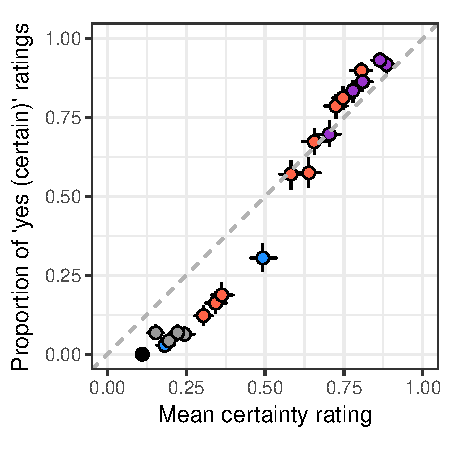
\includegraphics[width=.25\paperwidth]{../../results/compare-binary-nonbinary/graphs/projectivity}
\caption{Projectivity}
\end{subfigure}~\quad    
\begin{subfigure}{.33\textwidth}
\centering
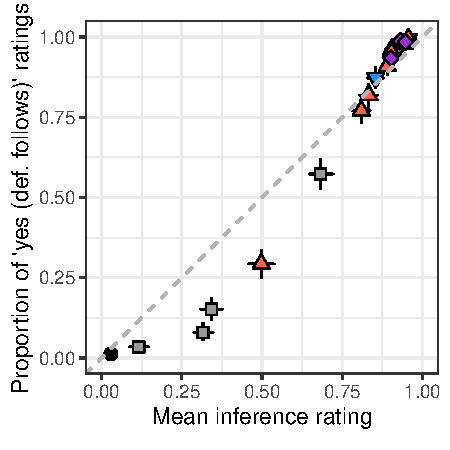
\includegraphics[width=.25\paperwidth]{../../results/compare-binary-nonbinary/graphs/entailment-inference}
\caption{Entailment: Inference}
\end{subfigure}~\quad   
\begin{subfigure}{.33\textwidth}
\centering
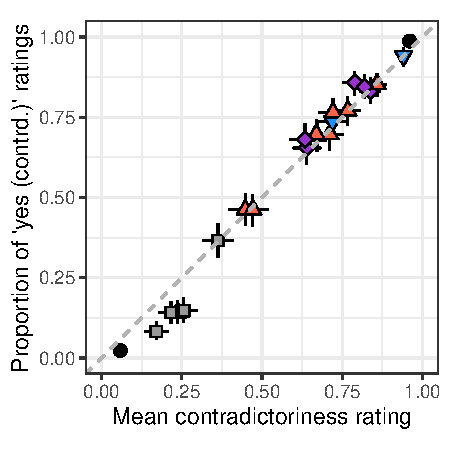
\includegraphics[width=.25\paperwidth]{../../results/compare-binary-nonbinary/graphs/entailment-contradictory}
\caption{Entailment: Contradictoriness}
\end{subfigure}    
   
\caption{Proportion of `yes' ratings in two-alternative forced choice task by mean ratings on gradient scale, with 95\% bootstrapped confidence intervals, collapsing over complement clauses. Controls are given in black, factive predicates in purple, veridical non-factive ones in light blue, optionally factive ones in orange and non-veridical non-factive ones in gray.}
\label{f-comparison}
\end{figure}

{\bf DESCRIBE BAYESIAN MODELS FOR BINARY DATA HERE}

\begin{itemize}

\item Experiment 1$'$: The CCs of all predicates were projective compared to the projectivity of the CC of {\em be right}, which were the least projective of all CCs, the CCs of the other 19 predicates were more projective. {\bf Describe model here, explain why we couldn't use the main clause controls as reference level: no variance.}

\end{itemize}


%\bibliographystyle{/Users/tonhauser.1/Library/Latex/cslipubs-natbib}
%\bibliography{/Users/tonhauser.1/Documents/bibliography}

\bibliographystyle{../cslipubs-natbib}
\bibliography{../bibliography}

\end{document}

